\documentclass[twoside]{book}

% Packages required by doxygen
\usepackage{fixltx2e}
\usepackage{calc}
\usepackage{doxygen}
\usepackage[export]{adjustbox} % also loads graphicx
\usepackage{graphicx}
\usepackage[utf8]{inputenc}
\usepackage{makeidx}
\usepackage{multicol}
\usepackage{multirow}
\PassOptionsToPackage{warn}{textcomp}
\usepackage{textcomp}
\usepackage[nointegrals]{wasysym}
\usepackage[table]{xcolor}

% Font selection
\usepackage[T1]{fontenc}
\usepackage[scaled=.90]{helvet}
\usepackage{courier}
\usepackage{amssymb}
\usepackage{sectsty}
\renewcommand{\familydefault}{\sfdefault}
\allsectionsfont{%
  \fontseries{bc}\selectfont%
  \color{darkgray}%
}
\renewcommand{\DoxyLabelFont}{%
  \fontseries{bc}\selectfont%
  \color{darkgray}%
}
\newcommand{\+}{\discretionary{\mbox{\scriptsize$\hookleftarrow$}}{}{}}

% Page & text layout
\usepackage{geometry}
\geometry{%
  a4paper,%
  top=2.5cm,%
  bottom=2.5cm,%
  left=2.5cm,%
  right=2.5cm%
}
\tolerance=750
\hfuzz=15pt
\hbadness=750
\setlength{\emergencystretch}{15pt}
\setlength{\parindent}{0cm}
\setlength{\parskip}{3ex plus 2ex minus 2ex}
\makeatletter
\renewcommand{\paragraph}{%
  \@startsection{paragraph}{4}{0ex}{-1.0ex}{1.0ex}{%
    \normalfont\normalsize\bfseries\SS@parafont%
  }%
}
\renewcommand{\subparagraph}{%
  \@startsection{subparagraph}{5}{0ex}{-1.0ex}{1.0ex}{%
    \normalfont\normalsize\bfseries\SS@subparafont%
  }%
}
\makeatother

% Headers & footers
\usepackage{fancyhdr}
\pagestyle{fancyplain}
\fancyhead[LE]{\fancyplain{}{\bfseries\thepage}}
\fancyhead[CE]{\fancyplain{}{}}
\fancyhead[RE]{\fancyplain{}{\bfseries\leftmark}}
\fancyhead[LO]{\fancyplain{}{\bfseries\rightmark}}
\fancyhead[CO]{\fancyplain{}{}}
\fancyhead[RO]{\fancyplain{}{\bfseries\thepage}}
\fancyfoot[LE]{\fancyplain{}{}}
\fancyfoot[CE]{\fancyplain{}{}}
\fancyfoot[RE]{\fancyplain{}{\bfseries\scriptsize Generated by Doxygen }}
\fancyfoot[LO]{\fancyplain{}{\bfseries\scriptsize Generated by Doxygen }}
\fancyfoot[CO]{\fancyplain{}{}}
\fancyfoot[RO]{\fancyplain{}{}}
\renewcommand{\footrulewidth}{0.4pt}
\renewcommand{\chaptermark}[1]{%
  \markboth{#1}{}%
}
\renewcommand{\sectionmark}[1]{%
  \markright{\thesection\ #1}%
}

% Indices & bibliography
\usepackage{natbib}
\usepackage[titles]{tocloft}
\setcounter{tocdepth}{3}
\setcounter{secnumdepth}{5}
\makeindex

% Hyperlinks (required, but should be loaded last)
\usepackage{ifpdf}
\ifpdf
  \usepackage[pdftex,pagebackref=true]{hyperref}
\else
  \usepackage[ps2pdf,pagebackref=true]{hyperref}
\fi
\hypersetup{%
  colorlinks=true,%
  linkcolor=blue,%
  citecolor=blue,%
  unicode%
}

% Custom commands
\newcommand{\clearemptydoublepage}{%
  \newpage{\pagestyle{empty}\cleardoublepage}%
}

\usepackage{caption}
\captionsetup{labelsep=space,justification=centering,font={bf},singlelinecheck=off,skip=4pt,position=top}

%===== C O N T E N T S =====

\begin{document}

% Titlepage & ToC
\hypersetup{pageanchor=false,
             bookmarksnumbered=true,
             pdfencoding=unicode
            }
\pagenumbering{alph}
\begin{titlepage}
\vspace*{7cm}
\begin{center}%
{\Large Heislab gruppe 17 }\\
\vspace*{1cm}
{\large Generated by Doxygen 1.8.13}\\
\end{center}
\end{titlepage}
\clearemptydoublepage
\pagenumbering{roman}
\tableofcontents
\clearemptydoublepage
\pagenumbering{arabic}
\hypersetup{pageanchor=true}

%--- Begin generated contents ---
\chapter{File Index}
\section{File List}
Here is a list of all files with brief descriptions\+:\begin{DoxyCompactList}
\item\contentsline{section}{source/\hyperlink{elevator_8c}{elevator.\+c} }{\pageref{elevator_8c}}{}
\item\contentsline{section}{source/\hyperlink{elevator_8h}{elevator.\+h} \\*Running elevator and updating states }{\pageref{elevator_8h}}{}
\item\contentsline{section}{source/\hyperlink{hardware_8h}{hardware.\+h} \\*Driver for the elevator hardware }{\pageref{hardware_8h}}{}
\item\contentsline{section}{source/\hyperlink{lights_8c}{lights.\+c} }{\pageref{lights_8c}}{}
\item\contentsline{section}{source/\hyperlink{lights_8h}{lights.\+h} \\*All functions handling the lights }{\pageref{lights_8h}}{}
\item\contentsline{section}{source/\hyperlink{main_8c}{main.\+c} }{\pageref{main_8c}}{}
\item\contentsline{section}{source/\hyperlink{orders_8c}{orders.\+c} }{\pageref{orders_8c}}{}
\item\contentsline{section}{source/\hyperlink{orders_8h}{orders.\+h} \\*Order handling, including the queue system }{\pageref{orders_8h}}{}
\item\contentsline{section}{source/\hyperlink{timer_8c}{timer.\+c} }{\pageref{timer_8c}}{}
\item\contentsline{section}{source/\hyperlink{timer_8h}{timer.\+h} \\*Time functions }{\pageref{timer_8h}}{}
\end{DoxyCompactList}

\chapter{File Documentation}
\hypertarget{elevator_8c}{}\section{source/elevator.c File Reference}
\label{elevator_8c}\index{source/elevator.\+c@{source/elevator.\+c}}
{\ttfamily \#include $<$stdio.\+h$>$}\newline
{\ttfamily \#include $<$stdlib.\+h$>$}\newline
{\ttfamily \#include \char`\"{}hardware.\+h\char`\"{}}\newline
{\ttfamily \#include \char`\"{}elevator.\+h\char`\"{}}\newline
{\ttfamily \#include \char`\"{}orders.\+h\char`\"{}}\newline
{\ttfamily \#include \char`\"{}lights.\+h\char`\"{}}\newline
{\ttfamily \#include \char`\"{}timer.\+h\char`\"{}}\newline
Include dependency graph for elevator.\+c\+:\nopagebreak
\begin{figure}[H]
\begin{center}
\leavevmode
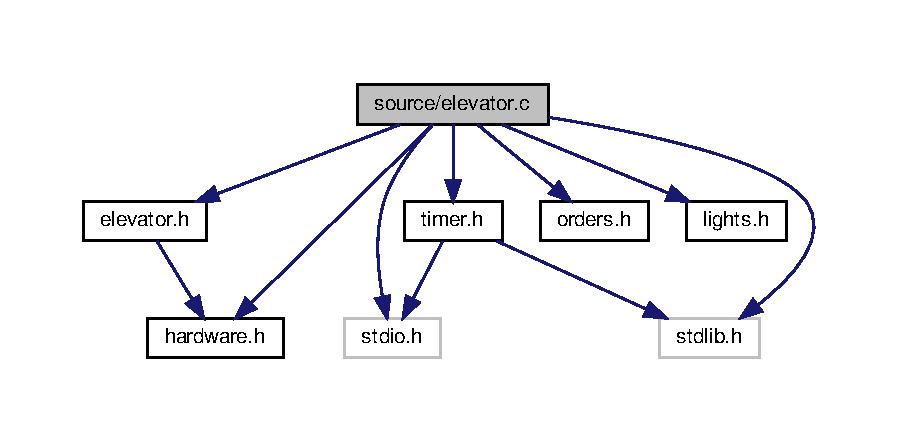
\includegraphics[width=350pt]{elevator_8c__incl}
\end{center}
\end{figure}
\subsection*{Functions}
\begin{DoxyCompactItemize}
\item 
int \hyperlink{elevator_8c_a0708c98c357f56f12e72a212e074cf79}{elevator\+\_\+get\+\_\+state} ()
\begin{DoxyCompactList}\small\item\em Gets the current state. \end{DoxyCompactList}\item 
void \hyperlink{elevator_8c_af76e1c65d1b9f5ad232c8402bdf72d0f}{elevator\+\_\+set\+\_\+state} (\hyperlink{elevator_8h_a59f51b412d7dfa606a5bf634db2aec32}{Current\+State} new\+\_\+state)
\begin{DoxyCompactList}\small\item\em Sets the state to {\ttfamily new\+\_\+state} . \end{DoxyCompactList}\item 
int \hyperlink{elevator_8c_ad785f5909121c35151e975eb671d4ef9}{elevator\+\_\+get\+\_\+current\+\_\+floor} ()
\begin{DoxyCompactList}\small\item\em Gets the current floor. \end{DoxyCompactList}\item 
int \hyperlink{elevator_8c_a45350efbdbe333355181a9d3338de783}{elevator\+\_\+get\+\_\+\+F\+L\+O\+O\+R\+\_\+\+C\+O\+U\+NT} ()
\begin{DoxyCompactList}\small\item\em Gets F\+L\+O\+O\+R\+\_\+\+C\+O\+U\+NT. \end{DoxyCompactList}\item 
int \hyperlink{elevator_8c_a087b64f5708f96b5c5c3e2d0c5bda1bc}{elevator\+\_\+get\+\_\+\+B\+U\+T\+T\+O\+N\+\_\+\+C\+O\+U\+NT} ()
\begin{DoxyCompactList}\small\item\em Gets B\+U\+T\+T\+O\+N\+\_\+\+C\+O\+U\+NT. \end{DoxyCompactList}\item 
int \hyperlink{elevator_8c_a98484defeb96eb259484ae8fac108484}{elevator\+\_\+one\+\_\+indexed\+\_\+floor\+\_\+number} ()
\begin{DoxyCompactList}\small\item\em Checks the floor number. \end{DoxyCompactList}\item 
void \hyperlink{elevator_8c_a768ffeedf962a239aa3cb8468742fd06}{elevator\+\_\+update\+\_\+current\+\_\+floor} ()
\begin{DoxyCompactList}\small\item\em Updates the current\+\_\+floor variable to the non-\/zero return value of \hyperlink{elevator_8h_a98484defeb96eb259484ae8fac108484}{elevator\+\_\+one\+\_\+indexed\+\_\+floor\+\_\+number()} \end{DoxyCompactList}\item 
void \hyperlink{elevator_8c_ac68447dda9a06fdb6c802303e170c98f}{elevator\+\_\+startup} ()
\begin{DoxyCompactList}\small\item\em Initialises the elevator and runs the elevator to the closest floor below. \end{DoxyCompactList}\item 
void \hyperlink{elevator_8c_a6da5e4f1c9ffccd598c4785e2fc68949}{elevator\+\_\+run\+\_\+elevator} ()
\begin{DoxyCompactList}\small\item\em Runs the elevator. \end{DoxyCompactList}\end{DoxyCompactItemize}
\subsection*{Variables}
\begin{DoxyCompactItemize}
\item 
int \hyperlink{elevator_8c_acb192fef68ecb95b51961bf64d80f71f}{F\+L\+O\+O\+R\+\_\+\+C\+O\+U\+NT} = 4
\item 
int \hyperlink{elevator_8c_aee37217a39699cf8c5bc77eb81315805}{B\+U\+T\+T\+O\+N\+\_\+\+C\+O\+U\+NT} = 3
\item 
int \hyperlink{elevator_8c_aafffa54a4465b20eac09db2c47fa54e2}{direction\+\_\+from\+\_\+last\+\_\+floor}
\item 
\hyperlink{elevator_8h_a59f51b412d7dfa606a5bf634db2aec32}{Current\+State} \hyperlink{elevator_8c_a46844f3a6da217c1aa4ddec219a46178}{state} = \hyperlink{elevator_8h_a59f51b412d7dfa606a5bf634db2aec32afd6a0e4343048b10646dd2976cc5ad18}{I\+D\+LE}
\end{DoxyCompactItemize}


\subsection{Function Documentation}
\mbox{\Hypertarget{elevator_8c_a087b64f5708f96b5c5c3e2d0c5bda1bc}\label{elevator_8c_a087b64f5708f96b5c5c3e2d0c5bda1bc}} 
\index{elevator.\+c@{elevator.\+c}!elevator\+\_\+get\+\_\+\+B\+U\+T\+T\+O\+N\+\_\+\+C\+O\+U\+NT@{elevator\+\_\+get\+\_\+\+B\+U\+T\+T\+O\+N\+\_\+\+C\+O\+U\+NT}}
\index{elevator\+\_\+get\+\_\+\+B\+U\+T\+T\+O\+N\+\_\+\+C\+O\+U\+NT@{elevator\+\_\+get\+\_\+\+B\+U\+T\+T\+O\+N\+\_\+\+C\+O\+U\+NT}!elevator.\+c@{elevator.\+c}}
\subsubsection{\texorpdfstring{elevator\+\_\+get\+\_\+\+B\+U\+T\+T\+O\+N\+\_\+\+C\+O\+U\+N\+T()}{elevator\_get\_BUTTON\_COUNT()}}
{\footnotesize\ttfamily int elevator\+\_\+get\+\_\+\+B\+U\+T\+T\+O\+N\+\_\+\+C\+O\+U\+NT (\begin{DoxyParamCaption}{ }\end{DoxyParamCaption})}



Gets B\+U\+T\+T\+O\+N\+\_\+\+C\+O\+U\+NT. 

\begin{DoxyReturn}{Returns}
Returns B\+U\+T\+T\+O\+N\+\_\+\+C\+O\+U\+NT. 
\end{DoxyReturn}


Definition at line 33 of file elevator.\+c.

\mbox{\Hypertarget{elevator_8c_ad785f5909121c35151e975eb671d4ef9}\label{elevator_8c_ad785f5909121c35151e975eb671d4ef9}} 
\index{elevator.\+c@{elevator.\+c}!elevator\+\_\+get\+\_\+current\+\_\+floor@{elevator\+\_\+get\+\_\+current\+\_\+floor}}
\index{elevator\+\_\+get\+\_\+current\+\_\+floor@{elevator\+\_\+get\+\_\+current\+\_\+floor}!elevator.\+c@{elevator.\+c}}
\subsubsection{\texorpdfstring{elevator\+\_\+get\+\_\+current\+\_\+floor()}{elevator\_get\_current\_floor()}}
{\footnotesize\ttfamily int elevator\+\_\+get\+\_\+current\+\_\+floor (\begin{DoxyParamCaption}{ }\end{DoxyParamCaption})}



Gets the current floor. 

\begin{DoxyReturn}{Returns}
Return current\+\_\+floor. 
\end{DoxyReturn}


Definition at line 25 of file elevator.\+c.

\mbox{\Hypertarget{elevator_8c_a45350efbdbe333355181a9d3338de783}\label{elevator_8c_a45350efbdbe333355181a9d3338de783}} 
\index{elevator.\+c@{elevator.\+c}!elevator\+\_\+get\+\_\+\+F\+L\+O\+O\+R\+\_\+\+C\+O\+U\+NT@{elevator\+\_\+get\+\_\+\+F\+L\+O\+O\+R\+\_\+\+C\+O\+U\+NT}}
\index{elevator\+\_\+get\+\_\+\+F\+L\+O\+O\+R\+\_\+\+C\+O\+U\+NT@{elevator\+\_\+get\+\_\+\+F\+L\+O\+O\+R\+\_\+\+C\+O\+U\+NT}!elevator.\+c@{elevator.\+c}}
\subsubsection{\texorpdfstring{elevator\+\_\+get\+\_\+\+F\+L\+O\+O\+R\+\_\+\+C\+O\+U\+N\+T()}{elevator\_get\_FLOOR\_COUNT()}}
{\footnotesize\ttfamily int elevator\+\_\+get\+\_\+\+F\+L\+O\+O\+R\+\_\+\+C\+O\+U\+NT (\begin{DoxyParamCaption}{ }\end{DoxyParamCaption})}



Gets F\+L\+O\+O\+R\+\_\+\+C\+O\+U\+NT. 

\begin{DoxyReturn}{Returns}
Returns F\+L\+O\+O\+R\+\_\+\+C\+O\+U\+NT. 
\end{DoxyReturn}


Definition at line 29 of file elevator.\+c.

\mbox{\Hypertarget{elevator_8c_a0708c98c357f56f12e72a212e074cf79}\label{elevator_8c_a0708c98c357f56f12e72a212e074cf79}} 
\index{elevator.\+c@{elevator.\+c}!elevator\+\_\+get\+\_\+state@{elevator\+\_\+get\+\_\+state}}
\index{elevator\+\_\+get\+\_\+state@{elevator\+\_\+get\+\_\+state}!elevator.\+c@{elevator.\+c}}
\subsubsection{\texorpdfstring{elevator\+\_\+get\+\_\+state()}{elevator\_get\_state()}}
{\footnotesize\ttfamily int elevator\+\_\+get\+\_\+state (\begin{DoxyParamCaption}{ }\end{DoxyParamCaption})}



Gets the current state. 

\begin{DoxyReturn}{Returns}
Return state. 
\end{DoxyReturn}


Definition at line 17 of file elevator.\+c.

\mbox{\Hypertarget{elevator_8c_a98484defeb96eb259484ae8fac108484}\label{elevator_8c_a98484defeb96eb259484ae8fac108484}} 
\index{elevator.\+c@{elevator.\+c}!elevator\+\_\+one\+\_\+indexed\+\_\+floor\+\_\+number@{elevator\+\_\+one\+\_\+indexed\+\_\+floor\+\_\+number}}
\index{elevator\+\_\+one\+\_\+indexed\+\_\+floor\+\_\+number@{elevator\+\_\+one\+\_\+indexed\+\_\+floor\+\_\+number}!elevator.\+c@{elevator.\+c}}
\subsubsection{\texorpdfstring{elevator\+\_\+one\+\_\+indexed\+\_\+floor\+\_\+number()}{elevator\_one\_indexed\_floor\_number()}}
{\footnotesize\ttfamily int elevator\+\_\+one\+\_\+indexed\+\_\+floor\+\_\+number (\begin{DoxyParamCaption}{ }\end{DoxyParamCaption})}



Checks the floor number. 

\begin{DoxyReturn}{Returns}
Return current floor. Return 0 if between floors. 
\end{DoxyReturn}


Definition at line 37 of file elevator.\+c.

\mbox{\Hypertarget{elevator_8c_a6da5e4f1c9ffccd598c4785e2fc68949}\label{elevator_8c_a6da5e4f1c9ffccd598c4785e2fc68949}} 
\index{elevator.\+c@{elevator.\+c}!elevator\+\_\+run\+\_\+elevator@{elevator\+\_\+run\+\_\+elevator}}
\index{elevator\+\_\+run\+\_\+elevator@{elevator\+\_\+run\+\_\+elevator}!elevator.\+c@{elevator.\+c}}
\subsubsection{\texorpdfstring{elevator\+\_\+run\+\_\+elevator()}{elevator\_run\_elevator()}}
{\footnotesize\ttfamily void elevator\+\_\+run\+\_\+elevator (\begin{DoxyParamCaption}{ }\end{DoxyParamCaption})}



Runs the elevator. 



Definition at line 68 of file elevator.\+c.

\mbox{\Hypertarget{elevator_8c_af76e1c65d1b9f5ad232c8402bdf72d0f}\label{elevator_8c_af76e1c65d1b9f5ad232c8402bdf72d0f}} 
\index{elevator.\+c@{elevator.\+c}!elevator\+\_\+set\+\_\+state@{elevator\+\_\+set\+\_\+state}}
\index{elevator\+\_\+set\+\_\+state@{elevator\+\_\+set\+\_\+state}!elevator.\+c@{elevator.\+c}}
\subsubsection{\texorpdfstring{elevator\+\_\+set\+\_\+state()}{elevator\_set\_state()}}
{\footnotesize\ttfamily void elevator\+\_\+set\+\_\+state (\begin{DoxyParamCaption}\item[{\hyperlink{elevator_8h_a59f51b412d7dfa606a5bf634db2aec32}{Current\+State}}]{new\+\_\+state }\end{DoxyParamCaption})}



Sets the state to {\ttfamily new\+\_\+state} . 


\begin{DoxyParams}{Parameters}
{\em new\+\_\+state} & \\
\hline
\end{DoxyParams}


Definition at line 21 of file elevator.\+c.

\mbox{\Hypertarget{elevator_8c_ac68447dda9a06fdb6c802303e170c98f}\label{elevator_8c_ac68447dda9a06fdb6c802303e170c98f}} 
\index{elevator.\+c@{elevator.\+c}!elevator\+\_\+startup@{elevator\+\_\+startup}}
\index{elevator\+\_\+startup@{elevator\+\_\+startup}!elevator.\+c@{elevator.\+c}}
\subsubsection{\texorpdfstring{elevator\+\_\+startup()}{elevator\_startup()}}
{\footnotesize\ttfamily void elevator\+\_\+startup (\begin{DoxyParamCaption}{ }\end{DoxyParamCaption})}



Initialises the elevator and runs the elevator to the closest floor below. 



Definition at line 53 of file elevator.\+c.

\mbox{\Hypertarget{elevator_8c_a768ffeedf962a239aa3cb8468742fd06}\label{elevator_8c_a768ffeedf962a239aa3cb8468742fd06}} 
\index{elevator.\+c@{elevator.\+c}!elevator\+\_\+update\+\_\+current\+\_\+floor@{elevator\+\_\+update\+\_\+current\+\_\+floor}}
\index{elevator\+\_\+update\+\_\+current\+\_\+floor@{elevator\+\_\+update\+\_\+current\+\_\+floor}!elevator.\+c@{elevator.\+c}}
\subsubsection{\texorpdfstring{elevator\+\_\+update\+\_\+current\+\_\+floor()}{elevator\_update\_current\_floor()}}
{\footnotesize\ttfamily void elevator\+\_\+update\+\_\+current\+\_\+floor (\begin{DoxyParamCaption}{ }\end{DoxyParamCaption})}



Updates the current\+\_\+floor variable to the non-\/zero return value of \hyperlink{elevator_8h_a98484defeb96eb259484ae8fac108484}{elevator\+\_\+one\+\_\+indexed\+\_\+floor\+\_\+number()} 



Definition at line 46 of file elevator.\+c.



\subsection{Variable Documentation}
\mbox{\Hypertarget{elevator_8c_aee37217a39699cf8c5bc77eb81315805}\label{elevator_8c_aee37217a39699cf8c5bc77eb81315805}} 
\index{elevator.\+c@{elevator.\+c}!B\+U\+T\+T\+O\+N\+\_\+\+C\+O\+U\+NT@{B\+U\+T\+T\+O\+N\+\_\+\+C\+O\+U\+NT}}
\index{B\+U\+T\+T\+O\+N\+\_\+\+C\+O\+U\+NT@{B\+U\+T\+T\+O\+N\+\_\+\+C\+O\+U\+NT}!elevator.\+c@{elevator.\+c}}
\subsubsection{\texorpdfstring{B\+U\+T\+T\+O\+N\+\_\+\+C\+O\+U\+NT}{BUTTON\_COUNT}}
{\footnotesize\ttfamily int B\+U\+T\+T\+O\+N\+\_\+\+C\+O\+U\+NT = 3}



Definition at line 10 of file elevator.\+c.

\mbox{\Hypertarget{elevator_8c_aafffa54a4465b20eac09db2c47fa54e2}\label{elevator_8c_aafffa54a4465b20eac09db2c47fa54e2}} 
\index{elevator.\+c@{elevator.\+c}!direction\+\_\+from\+\_\+last\+\_\+floor@{direction\+\_\+from\+\_\+last\+\_\+floor}}
\index{direction\+\_\+from\+\_\+last\+\_\+floor@{direction\+\_\+from\+\_\+last\+\_\+floor}!elevator.\+c@{elevator.\+c}}
\subsubsection{\texorpdfstring{direction\+\_\+from\+\_\+last\+\_\+floor}{direction\_from\_last\_floor}}
{\footnotesize\ttfamily int direction\+\_\+from\+\_\+last\+\_\+floor}



Definition at line 13 of file elevator.\+c.

\mbox{\Hypertarget{elevator_8c_acb192fef68ecb95b51961bf64d80f71f}\label{elevator_8c_acb192fef68ecb95b51961bf64d80f71f}} 
\index{elevator.\+c@{elevator.\+c}!F\+L\+O\+O\+R\+\_\+\+C\+O\+U\+NT@{F\+L\+O\+O\+R\+\_\+\+C\+O\+U\+NT}}
\index{F\+L\+O\+O\+R\+\_\+\+C\+O\+U\+NT@{F\+L\+O\+O\+R\+\_\+\+C\+O\+U\+NT}!elevator.\+c@{elevator.\+c}}
\subsubsection{\texorpdfstring{F\+L\+O\+O\+R\+\_\+\+C\+O\+U\+NT}{FLOOR\_COUNT}}
{\footnotesize\ttfamily int F\+L\+O\+O\+R\+\_\+\+C\+O\+U\+NT = 4}



Definition at line 9 of file elevator.\+c.

\mbox{\Hypertarget{elevator_8c_a46844f3a6da217c1aa4ddec219a46178}\label{elevator_8c_a46844f3a6da217c1aa4ddec219a46178}} 
\index{elevator.\+c@{elevator.\+c}!state@{state}}
\index{state@{state}!elevator.\+c@{elevator.\+c}}
\subsubsection{\texorpdfstring{state}{state}}
{\footnotesize\ttfamily \hyperlink{elevator_8h_a59f51b412d7dfa606a5bf634db2aec32}{Current\+State} state = \hyperlink{elevator_8h_a59f51b412d7dfa606a5bf634db2aec32afd6a0e4343048b10646dd2976cc5ad18}{I\+D\+LE}}



Definition at line 15 of file elevator.\+c.


\hypertarget{elevator_8h}{}\section{source/elevator.h File Reference}
\label{elevator_8h}\index{source/elevator.\+h@{source/elevator.\+h}}


Running elevator and updating states.  


{\ttfamily \#include \char`\"{}hardware.\+h\char`\"{}}\newline
Include dependency graph for elevator.\+h\+:\nopagebreak
\begin{figure}[H]
\begin{center}
\leavevmode
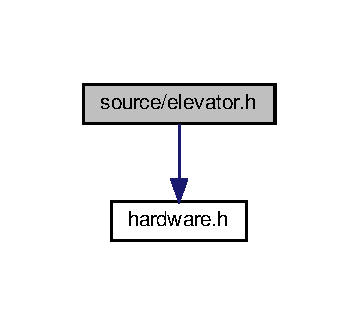
\includegraphics[width=172pt]{elevator_8h__incl}
\end{center}
\end{figure}
This graph shows which files directly or indirectly include this file\+:
\nopagebreak
\begin{figure}[H]
\begin{center}
\leavevmode
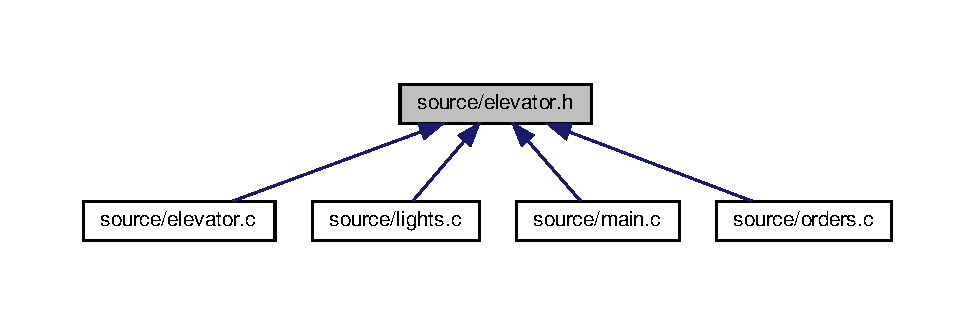
\includegraphics[width=350pt]{elevator_8h__dep__incl}
\end{center}
\end{figure}
\subsection*{Enumerations}
\begin{DoxyCompactItemize}
\item 
enum \hyperlink{elevator_8h_a59f51b412d7dfa606a5bf634db2aec32}{Current\+State} \{ \newline
\hyperlink{elevator_8h_a59f51b412d7dfa606a5bf634db2aec32afd6a0e4343048b10646dd2976cc5ad18}{I\+D\+LE}, 
\hyperlink{elevator_8h_a59f51b412d7dfa606a5bf634db2aec32a1061be6c3fb88d32829cba6f6b2be304}{R\+U\+N\+N\+I\+NG}, 
\hyperlink{elevator_8h_a59f51b412d7dfa606a5bf634db2aec32a56a92b9980c854fa6e488ffeb6a2844b}{E\+M\+E\+R\+G\+E\+N\+C\+Y\+\_\+\+S\+T\+OP}, 
\hyperlink{elevator_8h_a59f51b412d7dfa606a5bf634db2aec32ab5c63c54204a3c25d5ff88ea4d1d8336}{F\+L\+O\+OR}, 
\newline
\hyperlink{elevator_8h_a59f51b412d7dfa606a5bf634db2aec32aa51ed33c0d1a1bef96fd12d104261d95}{O\+B\+S\+T\+R\+U\+C\+T\+ED}
 \}\begin{DoxyCompactList}\small\item\em The possible states of the elevator. \end{DoxyCompactList}
\item 
enum \hyperlink{elevator_8h_ab332af6e5749eb14fb0761f0b0ea1cc2}{Order\+State} \{ \hyperlink{elevator_8h_ab332af6e5749eb14fb0761f0b0ea1cc2aba595d8bca8bc5e67c37c0a9d89becfa}{UP} = 1, 
\hyperlink{elevator_8h_ab332af6e5749eb14fb0761f0b0ea1cc2a9b0b4a95b99523966e0e34ffdadac9da}{D\+O\+WN}, 
\hyperlink{elevator_8h_ab332af6e5749eb14fb0761f0b0ea1cc2af9911bf84e010a42a26d0b6d9fccde56}{B\+O\+T\+H\+\_\+\+O\+R\+\_\+\+C\+AB}
 \}\begin{DoxyCompactList}\small\item\em The possible order types. \end{DoxyCompactList}
\end{DoxyCompactItemize}
\subsection*{Functions}
\begin{DoxyCompactItemize}
\item 
int \hyperlink{elevator_8h_a92ebb11dc8ea206c073a3509f413f513}{get\+\_\+state} ()
\begin{DoxyCompactList}\small\item\em Gets the current state. \end{DoxyCompactList}\item 
void \hyperlink{elevator_8h_aaf9bfa44cd72fb017ce630879140fd4f}{set\+\_\+state} (\hyperlink{elevator_8h_a59f51b412d7dfa606a5bf634db2aec32}{Current\+State} new\+\_\+state)
\begin{DoxyCompactList}\small\item\em Sets the state to {\ttfamily new\+\_\+state} . \end{DoxyCompactList}\item 
int \hyperlink{elevator_8h_a72be1591c37ccc47bcddab6e87a729b8}{get\+\_\+current\+\_\+floor} ()
\begin{DoxyCompactList}\small\item\em Gets the current floor. \end{DoxyCompactList}\item 
int \hyperlink{elevator_8h_a7f4b70feaa92b8a1ca3095ecc8a7cdb3}{get\+\_\+\+F\+L\+O\+O\+R\+\_\+\+C\+O\+U\+NT} ()
\begin{DoxyCompactList}\small\item\em Gets F\+L\+O\+O\+R\+\_\+\+C\+O\+U\+NT. \end{DoxyCompactList}\item 
int \hyperlink{elevator_8h_ab9a12b9b0714983a20e36429bb74643e}{get\+\_\+\+B\+U\+T\+T\+O\+N\+\_\+\+C\+O\+U\+NT} ()
\begin{DoxyCompactList}\small\item\em Gets B\+U\+T\+T\+O\+N\+\_\+\+C\+O\+U\+NT. \end{DoxyCompactList}\item 
int \hyperlink{elevator_8h_acbce1b7b0ebdde9d658511436d2a20bc}{check\+\_\+floor\+\_\+number} ()
\begin{DoxyCompactList}\small\item\em Checks the floor number. \end{DoxyCompactList}\item 
void \hyperlink{elevator_8h_a01ba2d8dfbbfa8f6c6fab7372f751eda}{update\+\_\+current\+\_\+floor} ()
\begin{DoxyCompactList}\small\item\em Updates the current\+\_\+floor variable to the non-\/zero return value of \hyperlink{elevator_8h_acbce1b7b0ebdde9d658511436d2a20bc}{check\+\_\+floor\+\_\+number()} \end{DoxyCompactList}\item 
void \hyperlink{elevator_8h_ac68447dda9a06fdb6c802303e170c98f}{elevator\+\_\+startup} ()
\begin{DoxyCompactList}\small\item\em Initialises the elevator and runs the elevator to the closest floor below. \end{DoxyCompactList}\item 
void \hyperlink{elevator_8h_a1690f0043d0c268acfba38c6c73cedb5}{run\+\_\+elevator} ()
\begin{DoxyCompactList}\small\item\em Runs the elevator. \end{DoxyCompactList}\end{DoxyCompactItemize}


\subsection{Detailed Description}
Running elevator and updating states. 



\subsection{Enumeration Type Documentation}
\mbox{\Hypertarget{elevator_8h_a59f51b412d7dfa606a5bf634db2aec32}\label{elevator_8h_a59f51b412d7dfa606a5bf634db2aec32}} 
\index{elevator.\+h@{elevator.\+h}!Current\+State@{Current\+State}}
\index{Current\+State@{Current\+State}!elevator.\+h@{elevator.\+h}}
\subsubsection{\texorpdfstring{Current\+State}{CurrentState}}
{\footnotesize\ttfamily enum \hyperlink{elevator_8h_a59f51b412d7dfa606a5bf634db2aec32}{Current\+State}}



The possible states of the elevator. 

\begin{DoxyEnumFields}{Enumerator}
\raisebox{\heightof{T}}[0pt][0pt]{\index{I\+D\+LE@{I\+D\+LE}!elevator.\+h@{elevator.\+h}}\index{elevator.\+h@{elevator.\+h}!I\+D\+LE@{I\+D\+LE}}}\mbox{\Hypertarget{elevator_8h_a59f51b412d7dfa606a5bf634db2aec32afd6a0e4343048b10646dd2976cc5ad18}\label{elevator_8h_a59f51b412d7dfa606a5bf634db2aec32afd6a0e4343048b10646dd2976cc5ad18}} 
I\+D\+LE&\\
\hline

\raisebox{\heightof{T}}[0pt][0pt]{\index{R\+U\+N\+N\+I\+NG@{R\+U\+N\+N\+I\+NG}!elevator.\+h@{elevator.\+h}}\index{elevator.\+h@{elevator.\+h}!R\+U\+N\+N\+I\+NG@{R\+U\+N\+N\+I\+NG}}}\mbox{\Hypertarget{elevator_8h_a59f51b412d7dfa606a5bf634db2aec32a1061be6c3fb88d32829cba6f6b2be304}\label{elevator_8h_a59f51b412d7dfa606a5bf634db2aec32a1061be6c3fb88d32829cba6f6b2be304}} 
R\+U\+N\+N\+I\+NG&\\
\hline

\raisebox{\heightof{T}}[0pt][0pt]{\index{E\+M\+E\+R\+G\+E\+N\+C\+Y\+\_\+\+S\+T\+OP@{E\+M\+E\+R\+G\+E\+N\+C\+Y\+\_\+\+S\+T\+OP}!elevator.\+h@{elevator.\+h}}\index{elevator.\+h@{elevator.\+h}!E\+M\+E\+R\+G\+E\+N\+C\+Y\+\_\+\+S\+T\+OP@{E\+M\+E\+R\+G\+E\+N\+C\+Y\+\_\+\+S\+T\+OP}}}\mbox{\Hypertarget{elevator_8h_a59f51b412d7dfa606a5bf634db2aec32a56a92b9980c854fa6e488ffeb6a2844b}\label{elevator_8h_a59f51b412d7dfa606a5bf634db2aec32a56a92b9980c854fa6e488ffeb6a2844b}} 
E\+M\+E\+R\+G\+E\+N\+C\+Y\+\_\+\+S\+T\+OP&\\
\hline

\raisebox{\heightof{T}}[0pt][0pt]{\index{F\+L\+O\+OR@{F\+L\+O\+OR}!elevator.\+h@{elevator.\+h}}\index{elevator.\+h@{elevator.\+h}!F\+L\+O\+OR@{F\+L\+O\+OR}}}\mbox{\Hypertarget{elevator_8h_a59f51b412d7dfa606a5bf634db2aec32ab5c63c54204a3c25d5ff88ea4d1d8336}\label{elevator_8h_a59f51b412d7dfa606a5bf634db2aec32ab5c63c54204a3c25d5ff88ea4d1d8336}} 
F\+L\+O\+OR&\\
\hline

\raisebox{\heightof{T}}[0pt][0pt]{\index{O\+B\+S\+T\+R\+U\+C\+T\+ED@{O\+B\+S\+T\+R\+U\+C\+T\+ED}!elevator.\+h@{elevator.\+h}}\index{elevator.\+h@{elevator.\+h}!O\+B\+S\+T\+R\+U\+C\+T\+ED@{O\+B\+S\+T\+R\+U\+C\+T\+ED}}}\mbox{\Hypertarget{elevator_8h_a59f51b412d7dfa606a5bf634db2aec32aa51ed33c0d1a1bef96fd12d104261d95}\label{elevator_8h_a59f51b412d7dfa606a5bf634db2aec32aa51ed33c0d1a1bef96fd12d104261d95}} 
O\+B\+S\+T\+R\+U\+C\+T\+ED&\\
\hline

\end{DoxyEnumFields}


Definition at line 12 of file elevator.\+h.

\mbox{\Hypertarget{elevator_8h_ab332af6e5749eb14fb0761f0b0ea1cc2}\label{elevator_8h_ab332af6e5749eb14fb0761f0b0ea1cc2}} 
\index{elevator.\+h@{elevator.\+h}!Order\+State@{Order\+State}}
\index{Order\+State@{Order\+State}!elevator.\+h@{elevator.\+h}}
\subsubsection{\texorpdfstring{Order\+State}{OrderState}}
{\footnotesize\ttfamily enum \hyperlink{elevator_8h_ab332af6e5749eb14fb0761f0b0ea1cc2}{Order\+State}}



The possible order types. 

\begin{DoxyEnumFields}{Enumerator}
\raisebox{\heightof{T}}[0pt][0pt]{\index{UP@{UP}!elevator.\+h@{elevator.\+h}}\index{elevator.\+h@{elevator.\+h}!UP@{UP}}}\mbox{\Hypertarget{elevator_8h_ab332af6e5749eb14fb0761f0b0ea1cc2aba595d8bca8bc5e67c37c0a9d89becfa}\label{elevator_8h_ab332af6e5749eb14fb0761f0b0ea1cc2aba595d8bca8bc5e67c37c0a9d89becfa}} 
UP&\\
\hline

\raisebox{\heightof{T}}[0pt][0pt]{\index{D\+O\+WN@{D\+O\+WN}!elevator.\+h@{elevator.\+h}}\index{elevator.\+h@{elevator.\+h}!D\+O\+WN@{D\+O\+WN}}}\mbox{\Hypertarget{elevator_8h_ab332af6e5749eb14fb0761f0b0ea1cc2a9b0b4a95b99523966e0e34ffdadac9da}\label{elevator_8h_ab332af6e5749eb14fb0761f0b0ea1cc2a9b0b4a95b99523966e0e34ffdadac9da}} 
D\+O\+WN&\\
\hline

\raisebox{\heightof{T}}[0pt][0pt]{\index{B\+O\+T\+H\+\_\+\+O\+R\+\_\+\+C\+AB@{B\+O\+T\+H\+\_\+\+O\+R\+\_\+\+C\+AB}!elevator.\+h@{elevator.\+h}}\index{elevator.\+h@{elevator.\+h}!B\+O\+T\+H\+\_\+\+O\+R\+\_\+\+C\+AB@{B\+O\+T\+H\+\_\+\+O\+R\+\_\+\+C\+AB}}}\mbox{\Hypertarget{elevator_8h_ab332af6e5749eb14fb0761f0b0ea1cc2af9911bf84e010a42a26d0b6d9fccde56}\label{elevator_8h_ab332af6e5749eb14fb0761f0b0ea1cc2af9911bf84e010a42a26d0b6d9fccde56}} 
B\+O\+T\+H\+\_\+\+O\+R\+\_\+\+C\+AB&\\
\hline

\end{DoxyEnumFields}


Definition at line 23 of file elevator.\+h.



\subsection{Function Documentation}
\mbox{\Hypertarget{elevator_8h_acbce1b7b0ebdde9d658511436d2a20bc}\label{elevator_8h_acbce1b7b0ebdde9d658511436d2a20bc}} 
\index{elevator.\+h@{elevator.\+h}!check\+\_\+floor\+\_\+number@{check\+\_\+floor\+\_\+number}}
\index{check\+\_\+floor\+\_\+number@{check\+\_\+floor\+\_\+number}!elevator.\+h@{elevator.\+h}}
\subsubsection{\texorpdfstring{check\+\_\+floor\+\_\+number()}{check\_floor\_number()}}
{\footnotesize\ttfamily int check\+\_\+floor\+\_\+number (\begin{DoxyParamCaption}{ }\end{DoxyParamCaption})}



Checks the floor number. 

\begin{DoxyReturn}{Returns}
Return current floor. Return 0 if between floors. 
\end{DoxyReturn}


Definition at line 37 of file elevator.\+c.

\mbox{\Hypertarget{elevator_8h_ac68447dda9a06fdb6c802303e170c98f}\label{elevator_8h_ac68447dda9a06fdb6c802303e170c98f}} 
\index{elevator.\+h@{elevator.\+h}!elevator\+\_\+startup@{elevator\+\_\+startup}}
\index{elevator\+\_\+startup@{elevator\+\_\+startup}!elevator.\+h@{elevator.\+h}}
\subsubsection{\texorpdfstring{elevator\+\_\+startup()}{elevator\_startup()}}
{\footnotesize\ttfamily void elevator\+\_\+startup (\begin{DoxyParamCaption}{ }\end{DoxyParamCaption})}



Initialises the elevator and runs the elevator to the closest floor below. 



Definition at line 53 of file elevator.\+c.

\mbox{\Hypertarget{elevator_8h_ab9a12b9b0714983a20e36429bb74643e}\label{elevator_8h_ab9a12b9b0714983a20e36429bb74643e}} 
\index{elevator.\+h@{elevator.\+h}!get\+\_\+\+B\+U\+T\+T\+O\+N\+\_\+\+C\+O\+U\+NT@{get\+\_\+\+B\+U\+T\+T\+O\+N\+\_\+\+C\+O\+U\+NT}}
\index{get\+\_\+\+B\+U\+T\+T\+O\+N\+\_\+\+C\+O\+U\+NT@{get\+\_\+\+B\+U\+T\+T\+O\+N\+\_\+\+C\+O\+U\+NT}!elevator.\+h@{elevator.\+h}}
\subsubsection{\texorpdfstring{get\+\_\+\+B\+U\+T\+T\+O\+N\+\_\+\+C\+O\+U\+N\+T()}{get\_BUTTON\_COUNT()}}
{\footnotesize\ttfamily int get\+\_\+\+B\+U\+T\+T\+O\+N\+\_\+\+C\+O\+U\+NT (\begin{DoxyParamCaption}{ }\end{DoxyParamCaption})}



Gets B\+U\+T\+T\+O\+N\+\_\+\+C\+O\+U\+NT. 

\begin{DoxyReturn}{Returns}
Returns B\+U\+T\+T\+O\+N\+\_\+\+C\+O\+U\+NT. 
\end{DoxyReturn}


Definition at line 33 of file elevator.\+c.

\mbox{\Hypertarget{elevator_8h_a72be1591c37ccc47bcddab6e87a729b8}\label{elevator_8h_a72be1591c37ccc47bcddab6e87a729b8}} 
\index{elevator.\+h@{elevator.\+h}!get\+\_\+current\+\_\+floor@{get\+\_\+current\+\_\+floor}}
\index{get\+\_\+current\+\_\+floor@{get\+\_\+current\+\_\+floor}!elevator.\+h@{elevator.\+h}}
\subsubsection{\texorpdfstring{get\+\_\+current\+\_\+floor()}{get\_current\_floor()}}
{\footnotesize\ttfamily int get\+\_\+current\+\_\+floor (\begin{DoxyParamCaption}{ }\end{DoxyParamCaption})}



Gets the current floor. 

\begin{DoxyReturn}{Returns}
Return current\+\_\+floor. 
\end{DoxyReturn}


Definition at line 25 of file elevator.\+c.

\mbox{\Hypertarget{elevator_8h_a7f4b70feaa92b8a1ca3095ecc8a7cdb3}\label{elevator_8h_a7f4b70feaa92b8a1ca3095ecc8a7cdb3}} 
\index{elevator.\+h@{elevator.\+h}!get\+\_\+\+F\+L\+O\+O\+R\+\_\+\+C\+O\+U\+NT@{get\+\_\+\+F\+L\+O\+O\+R\+\_\+\+C\+O\+U\+NT}}
\index{get\+\_\+\+F\+L\+O\+O\+R\+\_\+\+C\+O\+U\+NT@{get\+\_\+\+F\+L\+O\+O\+R\+\_\+\+C\+O\+U\+NT}!elevator.\+h@{elevator.\+h}}
\subsubsection{\texorpdfstring{get\+\_\+\+F\+L\+O\+O\+R\+\_\+\+C\+O\+U\+N\+T()}{get\_FLOOR\_COUNT()}}
{\footnotesize\ttfamily int get\+\_\+\+F\+L\+O\+O\+R\+\_\+\+C\+O\+U\+NT (\begin{DoxyParamCaption}{ }\end{DoxyParamCaption})}



Gets F\+L\+O\+O\+R\+\_\+\+C\+O\+U\+NT. 

\begin{DoxyReturn}{Returns}
Returns F\+L\+O\+O\+R\+\_\+\+C\+O\+U\+NT. 
\end{DoxyReturn}


Definition at line 29 of file elevator.\+c.

\mbox{\Hypertarget{elevator_8h_a92ebb11dc8ea206c073a3509f413f513}\label{elevator_8h_a92ebb11dc8ea206c073a3509f413f513}} 
\index{elevator.\+h@{elevator.\+h}!get\+\_\+state@{get\+\_\+state}}
\index{get\+\_\+state@{get\+\_\+state}!elevator.\+h@{elevator.\+h}}
\subsubsection{\texorpdfstring{get\+\_\+state()}{get\_state()}}
{\footnotesize\ttfamily int get\+\_\+state (\begin{DoxyParamCaption}{ }\end{DoxyParamCaption})}



Gets the current state. 

\begin{DoxyReturn}{Returns}
Return state. 
\end{DoxyReturn}


Definition at line 17 of file elevator.\+c.

\mbox{\Hypertarget{elevator_8h_a1690f0043d0c268acfba38c6c73cedb5}\label{elevator_8h_a1690f0043d0c268acfba38c6c73cedb5}} 
\index{elevator.\+h@{elevator.\+h}!run\+\_\+elevator@{run\+\_\+elevator}}
\index{run\+\_\+elevator@{run\+\_\+elevator}!elevator.\+h@{elevator.\+h}}
\subsubsection{\texorpdfstring{run\+\_\+elevator()}{run\_elevator()}}
{\footnotesize\ttfamily void run\+\_\+elevator (\begin{DoxyParamCaption}{ }\end{DoxyParamCaption})}



Runs the elevator. 



Definition at line 68 of file elevator.\+c.

\mbox{\Hypertarget{elevator_8h_aaf9bfa44cd72fb017ce630879140fd4f}\label{elevator_8h_aaf9bfa44cd72fb017ce630879140fd4f}} 
\index{elevator.\+h@{elevator.\+h}!set\+\_\+state@{set\+\_\+state}}
\index{set\+\_\+state@{set\+\_\+state}!elevator.\+h@{elevator.\+h}}
\subsubsection{\texorpdfstring{set\+\_\+state()}{set\_state()}}
{\footnotesize\ttfamily void set\+\_\+state (\begin{DoxyParamCaption}\item[{\hyperlink{elevator_8h_a59f51b412d7dfa606a5bf634db2aec32}{Current\+State}}]{new\+\_\+state }\end{DoxyParamCaption})}



Sets the state to {\ttfamily new\+\_\+state} . 


\begin{DoxyParams}{Parameters}
{\em new\+\_\+state} & \\
\hline
\end{DoxyParams}


Definition at line 21 of file elevator.\+c.

\mbox{\Hypertarget{elevator_8h_a01ba2d8dfbbfa8f6c6fab7372f751eda}\label{elevator_8h_a01ba2d8dfbbfa8f6c6fab7372f751eda}} 
\index{elevator.\+h@{elevator.\+h}!update\+\_\+current\+\_\+floor@{update\+\_\+current\+\_\+floor}}
\index{update\+\_\+current\+\_\+floor@{update\+\_\+current\+\_\+floor}!elevator.\+h@{elevator.\+h}}
\subsubsection{\texorpdfstring{update\+\_\+current\+\_\+floor()}{update\_current\_floor()}}
{\footnotesize\ttfamily void update\+\_\+current\+\_\+floor (\begin{DoxyParamCaption}{ }\end{DoxyParamCaption})}



Updates the current\+\_\+floor variable to the non-\/zero return value of \hyperlink{elevator_8h_acbce1b7b0ebdde9d658511436d2a20bc}{check\+\_\+floor\+\_\+number()} 



Definition at line 46 of file elevator.\+c.


\hypertarget{hardware_8h}{}\section{source/hardware.h File Reference}
\label{hardware_8h}\index{source/hardware.\+h@{source/hardware.\+h}}


Driver for the elevator hardware.  


This graph shows which files directly or indirectly include this file\+:\nopagebreak
\begin{figure}[H]
\begin{center}
\leavevmode
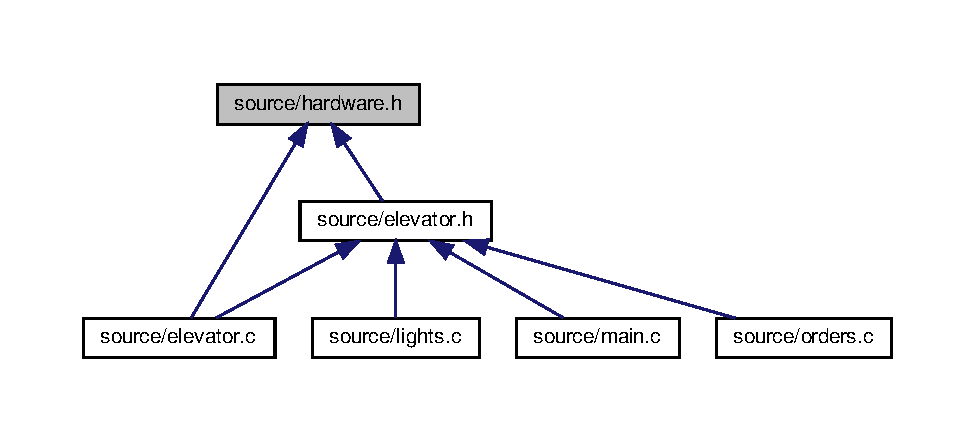
\includegraphics[width=350pt]{hardware_8h__dep__incl}
\end{center}
\end{figure}
\subsection*{Macros}
\begin{DoxyCompactItemize}
\item 
\#define \hyperlink{hardware_8h_ae9e42615eade15633bd8c03b7a271a00}{H\+A\+R\+D\+W\+A\+R\+E\+\_\+\+N\+U\+M\+B\+E\+R\+\_\+\+O\+F\+\_\+\+F\+L\+O\+O\+RS}~4
\end{DoxyCompactItemize}
\subsection*{Enumerations}
\begin{DoxyCompactItemize}
\item 
enum \hyperlink{hardware_8h_a2167c399a24df296afc432bcb88228af}{Hardware\+Movement} \{ \hyperlink{hardware_8h_a2167c399a24df296afc432bcb88228afaee0d800f6eabb40ed7fc57fdfa3956cf}{H\+A\+R\+D\+W\+A\+R\+E\+\_\+\+M\+O\+V\+E\+M\+E\+N\+T\+\_\+\+UP}, 
\hyperlink{hardware_8h_a2167c399a24df296afc432bcb88228afa0c5a09f827e65f3bb650d478638dd1c6}{H\+A\+R\+D\+W\+A\+R\+E\+\_\+\+M\+O\+V\+E\+M\+E\+N\+T\+\_\+\+S\+T\+OP}, 
\hyperlink{hardware_8h_a2167c399a24df296afc432bcb88228afa1e24e10c9811fb49a390c4027444ab74}{H\+A\+R\+D\+W\+A\+R\+E\+\_\+\+M\+O\+V\+E\+M\+E\+N\+T\+\_\+\+D\+O\+WN}
 \}\begin{DoxyCompactList}\small\item\em Movement type used in {\ttfamily hardware\+\_\+command\+\_\+movement}. \end{DoxyCompactList}
\item 
enum \hyperlink{hardware_8h_a796a8de8ce0ae769d7dbd3327a7bdbe7}{Hardware\+Order} \{ \hyperlink{hardware_8h_a796a8de8ce0ae769d7dbd3327a7bdbe7a04897c42fba48a7634f124b54f2c2e86}{H\+A\+R\+D\+W\+A\+R\+E\+\_\+\+O\+R\+D\+E\+R\+\_\+\+UP}, 
\hyperlink{hardware_8h_a796a8de8ce0ae769d7dbd3327a7bdbe7a98a032e849f3efead8f35958cb8daeb6}{H\+A\+R\+D\+W\+A\+R\+E\+\_\+\+O\+R\+D\+E\+R\+\_\+\+I\+N\+S\+I\+DE}, 
\hyperlink{hardware_8h_a796a8de8ce0ae769d7dbd3327a7bdbe7acfd939b1a6090d92033d621630f85603}{H\+A\+R\+D\+W\+A\+R\+E\+\_\+\+O\+R\+D\+E\+R\+\_\+\+D\+O\+WN}
 \}\begin{DoxyCompactList}\small\item\em Order type used in {\ttfamily hardware\+\_\+read\+\_\+order} and in {\ttfamily hardware\+\_\+command\+\_\+order\+\_\+light}. \end{DoxyCompactList}
\end{DoxyCompactItemize}
\subsection*{Functions}
\begin{DoxyCompactItemize}
\item 
int \hyperlink{hardware_8h_a054b8fb8768311d46be58d6a4890d771}{hardware\+\_\+init} ()
\begin{DoxyCompactList}\small\item\em Initializes the elevator control hardware. Must be called once before other calls to the elevator hardware driver. \end{DoxyCompactList}\item 
void \hyperlink{hardware_8h_a01de081ef0510a111053c18cd31afa27}{hardware\+\_\+command\+\_\+movement} (\hyperlink{hardware_8h_a2167c399a24df296afc432bcb88228af}{Hardware\+Movement} movement)
\begin{DoxyCompactList}\small\item\em Commands the elevator to either move up or down, or commands it to halt. \end{DoxyCompactList}\item 
int \hyperlink{hardware_8h_a4a77b27c86675c00b513db3445966804}{hardware\+\_\+read\+\_\+stop\+\_\+signal} ()
\begin{DoxyCompactList}\small\item\em Polls the hardware for the current stop signal. \end{DoxyCompactList}\item 
int \hyperlink{hardware_8h_a459fe57a3ee4bc2a28e8a15b2ab14c2d}{hardware\+\_\+read\+\_\+obstruction\+\_\+signal} ()
\begin{DoxyCompactList}\small\item\em Polls the hardware for the current obstruction signal. \end{DoxyCompactList}\item 
int \hyperlink{hardware_8h_ab048489e6302bb5604aad753f2d7d501}{hardware\+\_\+read\+\_\+floor\+\_\+sensor} (int floor)
\begin{DoxyCompactList}\small\item\em Polls the floor sensor for the given {\ttfamily floor}. \end{DoxyCompactList}\item 
int \hyperlink{hardware_8h_a87917f3aa093fb46ca821a400d011ee8}{hardware\+\_\+read\+\_\+order} (int floor, \hyperlink{hardware_8h_a796a8de8ce0ae769d7dbd3327a7bdbe7}{Hardware\+Order} order\+\_\+type)
\begin{DoxyCompactList}\small\item\em Polls the hardware for the status of orders from floor {\ttfamily floor} of type {\ttfamily order\+\_\+type}. \end{DoxyCompactList}\item 
void \hyperlink{hardware_8h_a80d99ddaa8e7b58c9a88b60ea553c1b6}{hardware\+\_\+command\+\_\+door\+\_\+open} (int door\+\_\+open)
\begin{DoxyCompactList}\small\item\em Commands the hardware to open-\/ or close the elevator door. \end{DoxyCompactList}\item 
void \hyperlink{hardware_8h_a407a6ec035ba357de6aa0fbe55501d1e}{hardware\+\_\+command\+\_\+floor\+\_\+indicator\+\_\+on} (int floor)
\begin{DoxyCompactList}\small\item\em Commands the hardware to turn on the floor indicator for {\ttfamily floor}. All indicators all mutually exclusive; other indicator lights will turn off. \end{DoxyCompactList}\item 
void \hyperlink{hardware_8h_aa75b3ac17f72b25946414f48d0063a10}{hardware\+\_\+command\+\_\+stop\+\_\+light} (int on)
\begin{DoxyCompactList}\small\item\em Sets the light in the panel stop button. \end{DoxyCompactList}\item 
void \hyperlink{hardware_8h_aa9b33faa52f0ec5b614d3e7dc05be140}{hardware\+\_\+command\+\_\+order\+\_\+light} (int floor, \hyperlink{hardware_8h_a796a8de8ce0ae769d7dbd3327a7bdbe7}{Hardware\+Order} order\+\_\+type, int on)
\begin{DoxyCompactList}\small\item\em Sets the light in a button corresponding to an order of type {\ttfamily order\+\_\+type}, at floor {\ttfamily floor}. \end{DoxyCompactList}\end{DoxyCompactItemize}


\subsection{Detailed Description}
Driver for the elevator hardware. 

Neatly wraps up Martin Korsgaard\textquotesingle{}s spaghetti from 2006 ;)

Kolbjørn Austreng 

\subsection{Macro Definition Documentation}
\mbox{\Hypertarget{hardware_8h_ae9e42615eade15633bd8c03b7a271a00}\label{hardware_8h_ae9e42615eade15633bd8c03b7a271a00}} 
\index{hardware.\+h@{hardware.\+h}!H\+A\+R\+D\+W\+A\+R\+E\+\_\+\+N\+U\+M\+B\+E\+R\+\_\+\+O\+F\+\_\+\+F\+L\+O\+O\+RS@{H\+A\+R\+D\+W\+A\+R\+E\+\_\+\+N\+U\+M\+B\+E\+R\+\_\+\+O\+F\+\_\+\+F\+L\+O\+O\+RS}}
\index{H\+A\+R\+D\+W\+A\+R\+E\+\_\+\+N\+U\+M\+B\+E\+R\+\_\+\+O\+F\+\_\+\+F\+L\+O\+O\+RS@{H\+A\+R\+D\+W\+A\+R\+E\+\_\+\+N\+U\+M\+B\+E\+R\+\_\+\+O\+F\+\_\+\+F\+L\+O\+O\+RS}!hardware.\+h@{hardware.\+h}}
\subsubsection{\texorpdfstring{H\+A\+R\+D\+W\+A\+R\+E\+\_\+\+N\+U\+M\+B\+E\+R\+\_\+\+O\+F\+\_\+\+F\+L\+O\+O\+RS}{HARDWARE\_NUMBER\_OF\_FLOORS}}
{\footnotesize\ttfamily \#define H\+A\+R\+D\+W\+A\+R\+E\+\_\+\+N\+U\+M\+B\+E\+R\+\_\+\+O\+F\+\_\+\+F\+L\+O\+O\+RS~4}



Definition at line 12 of file hardware.\+h.



\subsection{Enumeration Type Documentation}
\mbox{\Hypertarget{hardware_8h_a2167c399a24df296afc432bcb88228af}\label{hardware_8h_a2167c399a24df296afc432bcb88228af}} 
\index{hardware.\+h@{hardware.\+h}!Hardware\+Movement@{Hardware\+Movement}}
\index{Hardware\+Movement@{Hardware\+Movement}!hardware.\+h@{hardware.\+h}}
\subsubsection{\texorpdfstring{Hardware\+Movement}{HardwareMovement}}
{\footnotesize\ttfamily enum \hyperlink{hardware_8h_a2167c399a24df296afc432bcb88228af}{Hardware\+Movement}}



Movement type used in {\ttfamily hardware\+\_\+command\+\_\+movement}. 

\begin{DoxyEnumFields}{Enumerator}
\raisebox{\heightof{T}}[0pt][0pt]{\index{H\+A\+R\+D\+W\+A\+R\+E\+\_\+\+M\+O\+V\+E\+M\+E\+N\+T\+\_\+\+UP@{H\+A\+R\+D\+W\+A\+R\+E\+\_\+\+M\+O\+V\+E\+M\+E\+N\+T\+\_\+\+UP}!hardware.\+h@{hardware.\+h}}\index{hardware.\+h@{hardware.\+h}!H\+A\+R\+D\+W\+A\+R\+E\+\_\+\+M\+O\+V\+E\+M\+E\+N\+T\+\_\+\+UP@{H\+A\+R\+D\+W\+A\+R\+E\+\_\+\+M\+O\+V\+E\+M\+E\+N\+T\+\_\+\+UP}}}\mbox{\Hypertarget{hardware_8h_a2167c399a24df296afc432bcb88228afaee0d800f6eabb40ed7fc57fdfa3956cf}\label{hardware_8h_a2167c399a24df296afc432bcb88228afaee0d800f6eabb40ed7fc57fdfa3956cf}} 
H\+A\+R\+D\+W\+A\+R\+E\+\_\+\+M\+O\+V\+E\+M\+E\+N\+T\+\_\+\+UP&\\
\hline

\raisebox{\heightof{T}}[0pt][0pt]{\index{H\+A\+R\+D\+W\+A\+R\+E\+\_\+\+M\+O\+V\+E\+M\+E\+N\+T\+\_\+\+S\+T\+OP@{H\+A\+R\+D\+W\+A\+R\+E\+\_\+\+M\+O\+V\+E\+M\+E\+N\+T\+\_\+\+S\+T\+OP}!hardware.\+h@{hardware.\+h}}\index{hardware.\+h@{hardware.\+h}!H\+A\+R\+D\+W\+A\+R\+E\+\_\+\+M\+O\+V\+E\+M\+E\+N\+T\+\_\+\+S\+T\+OP@{H\+A\+R\+D\+W\+A\+R\+E\+\_\+\+M\+O\+V\+E\+M\+E\+N\+T\+\_\+\+S\+T\+OP}}}\mbox{\Hypertarget{hardware_8h_a2167c399a24df296afc432bcb88228afa0c5a09f827e65f3bb650d478638dd1c6}\label{hardware_8h_a2167c399a24df296afc432bcb88228afa0c5a09f827e65f3bb650d478638dd1c6}} 
H\+A\+R\+D\+W\+A\+R\+E\+\_\+\+M\+O\+V\+E\+M\+E\+N\+T\+\_\+\+S\+T\+OP&\\
\hline

\raisebox{\heightof{T}}[0pt][0pt]{\index{H\+A\+R\+D\+W\+A\+R\+E\+\_\+\+M\+O\+V\+E\+M\+E\+N\+T\+\_\+\+D\+O\+WN@{H\+A\+R\+D\+W\+A\+R\+E\+\_\+\+M\+O\+V\+E\+M\+E\+N\+T\+\_\+\+D\+O\+WN}!hardware.\+h@{hardware.\+h}}\index{hardware.\+h@{hardware.\+h}!H\+A\+R\+D\+W\+A\+R\+E\+\_\+\+M\+O\+V\+E\+M\+E\+N\+T\+\_\+\+D\+O\+WN@{H\+A\+R\+D\+W\+A\+R\+E\+\_\+\+M\+O\+V\+E\+M\+E\+N\+T\+\_\+\+D\+O\+WN}}}\mbox{\Hypertarget{hardware_8h_a2167c399a24df296afc432bcb88228afa1e24e10c9811fb49a390c4027444ab74}\label{hardware_8h_a2167c399a24df296afc432bcb88228afa1e24e10c9811fb49a390c4027444ab74}} 
H\+A\+R\+D\+W\+A\+R\+E\+\_\+\+M\+O\+V\+E\+M\+E\+N\+T\+\_\+\+D\+O\+WN&\\
\hline

\end{DoxyEnumFields}


Definition at line 17 of file hardware.\+h.

\mbox{\Hypertarget{hardware_8h_a796a8de8ce0ae769d7dbd3327a7bdbe7}\label{hardware_8h_a796a8de8ce0ae769d7dbd3327a7bdbe7}} 
\index{hardware.\+h@{hardware.\+h}!Hardware\+Order@{Hardware\+Order}}
\index{Hardware\+Order@{Hardware\+Order}!hardware.\+h@{hardware.\+h}}
\subsubsection{\texorpdfstring{Hardware\+Order}{HardwareOrder}}
{\footnotesize\ttfamily enum \hyperlink{hardware_8h_a796a8de8ce0ae769d7dbd3327a7bdbe7}{Hardware\+Order}}



Order type used in {\ttfamily hardware\+\_\+read\+\_\+order} and in {\ttfamily hardware\+\_\+command\+\_\+order\+\_\+light}. 

\begin{DoxyEnumFields}{Enumerator}
\raisebox{\heightof{T}}[0pt][0pt]{\index{H\+A\+R\+D\+W\+A\+R\+E\+\_\+\+O\+R\+D\+E\+R\+\_\+\+UP@{H\+A\+R\+D\+W\+A\+R\+E\+\_\+\+O\+R\+D\+E\+R\+\_\+\+UP}!hardware.\+h@{hardware.\+h}}\index{hardware.\+h@{hardware.\+h}!H\+A\+R\+D\+W\+A\+R\+E\+\_\+\+O\+R\+D\+E\+R\+\_\+\+UP@{H\+A\+R\+D\+W\+A\+R\+E\+\_\+\+O\+R\+D\+E\+R\+\_\+\+UP}}}\mbox{\Hypertarget{hardware_8h_a796a8de8ce0ae769d7dbd3327a7bdbe7a04897c42fba48a7634f124b54f2c2e86}\label{hardware_8h_a796a8de8ce0ae769d7dbd3327a7bdbe7a04897c42fba48a7634f124b54f2c2e86}} 
H\+A\+R\+D\+W\+A\+R\+E\+\_\+\+O\+R\+D\+E\+R\+\_\+\+UP&\\
\hline

\raisebox{\heightof{T}}[0pt][0pt]{\index{H\+A\+R\+D\+W\+A\+R\+E\+\_\+\+O\+R\+D\+E\+R\+\_\+\+I\+N\+S\+I\+DE@{H\+A\+R\+D\+W\+A\+R\+E\+\_\+\+O\+R\+D\+E\+R\+\_\+\+I\+N\+S\+I\+DE}!hardware.\+h@{hardware.\+h}}\index{hardware.\+h@{hardware.\+h}!H\+A\+R\+D\+W\+A\+R\+E\+\_\+\+O\+R\+D\+E\+R\+\_\+\+I\+N\+S\+I\+DE@{H\+A\+R\+D\+W\+A\+R\+E\+\_\+\+O\+R\+D\+E\+R\+\_\+\+I\+N\+S\+I\+DE}}}\mbox{\Hypertarget{hardware_8h_a796a8de8ce0ae769d7dbd3327a7bdbe7a98a032e849f3efead8f35958cb8daeb6}\label{hardware_8h_a796a8de8ce0ae769d7dbd3327a7bdbe7a98a032e849f3efead8f35958cb8daeb6}} 
H\+A\+R\+D\+W\+A\+R\+E\+\_\+\+O\+R\+D\+E\+R\+\_\+\+I\+N\+S\+I\+DE&\\
\hline

\raisebox{\heightof{T}}[0pt][0pt]{\index{H\+A\+R\+D\+W\+A\+R\+E\+\_\+\+O\+R\+D\+E\+R\+\_\+\+D\+O\+WN@{H\+A\+R\+D\+W\+A\+R\+E\+\_\+\+O\+R\+D\+E\+R\+\_\+\+D\+O\+WN}!hardware.\+h@{hardware.\+h}}\index{hardware.\+h@{hardware.\+h}!H\+A\+R\+D\+W\+A\+R\+E\+\_\+\+O\+R\+D\+E\+R\+\_\+\+D\+O\+WN@{H\+A\+R\+D\+W\+A\+R\+E\+\_\+\+O\+R\+D\+E\+R\+\_\+\+D\+O\+WN}}}\mbox{\Hypertarget{hardware_8h_a796a8de8ce0ae769d7dbd3327a7bdbe7acfd939b1a6090d92033d621630f85603}\label{hardware_8h_a796a8de8ce0ae769d7dbd3327a7bdbe7acfd939b1a6090d92033d621630f85603}} 
H\+A\+R\+D\+W\+A\+R\+E\+\_\+\+O\+R\+D\+E\+R\+\_\+\+D\+O\+WN&\\
\hline

\end{DoxyEnumFields}


Definition at line 27 of file hardware.\+h.



\subsection{Function Documentation}
\mbox{\Hypertarget{hardware_8h_a80d99ddaa8e7b58c9a88b60ea553c1b6}\label{hardware_8h_a80d99ddaa8e7b58c9a88b60ea553c1b6}} 
\index{hardware.\+h@{hardware.\+h}!hardware\+\_\+command\+\_\+door\+\_\+open@{hardware\+\_\+command\+\_\+door\+\_\+open}}
\index{hardware\+\_\+command\+\_\+door\+\_\+open@{hardware\+\_\+command\+\_\+door\+\_\+open}!hardware.\+h@{hardware.\+h}}
\subsubsection{\texorpdfstring{hardware\+\_\+command\+\_\+door\+\_\+open()}{hardware\_command\_door\_open()}}
{\footnotesize\ttfamily void hardware\+\_\+command\+\_\+door\+\_\+open (\begin{DoxyParamCaption}\item[{int}]{door\+\_\+open }\end{DoxyParamCaption})}



Commands the hardware to open-\/ or close the elevator door. 


\begin{DoxyParams}{Parameters}
{\em door\+\_\+open} & A truthy value (non-\/zero) to open the door; 0 to close. \\
\hline
\end{DoxyParams}
\mbox{\Hypertarget{hardware_8h_a407a6ec035ba357de6aa0fbe55501d1e}\label{hardware_8h_a407a6ec035ba357de6aa0fbe55501d1e}} 
\index{hardware.\+h@{hardware.\+h}!hardware\+\_\+command\+\_\+floor\+\_\+indicator\+\_\+on@{hardware\+\_\+command\+\_\+floor\+\_\+indicator\+\_\+on}}
\index{hardware\+\_\+command\+\_\+floor\+\_\+indicator\+\_\+on@{hardware\+\_\+command\+\_\+floor\+\_\+indicator\+\_\+on}!hardware.\+h@{hardware.\+h}}
\subsubsection{\texorpdfstring{hardware\+\_\+command\+\_\+floor\+\_\+indicator\+\_\+on()}{hardware\_command\_floor\_indicator\_on()}}
{\footnotesize\ttfamily void hardware\+\_\+command\+\_\+floor\+\_\+indicator\+\_\+on (\begin{DoxyParamCaption}\item[{int}]{floor }\end{DoxyParamCaption})}



Commands the hardware to turn on the floor indicator for {\ttfamily floor}. All indicators all mutually exclusive; other indicator lights will turn off. 


\begin{DoxyParams}{Parameters}
{\em floor} & Floor to turn on the indicator for.\\
\hline
\end{DoxyParams}
\begin{DoxyWarning}{Warning}
Owing to peculiarities in the hardware construction, there will always be one indicator active. 
\end{DoxyWarning}
\mbox{\Hypertarget{hardware_8h_a01de081ef0510a111053c18cd31afa27}\label{hardware_8h_a01de081ef0510a111053c18cd31afa27}} 
\index{hardware.\+h@{hardware.\+h}!hardware\+\_\+command\+\_\+movement@{hardware\+\_\+command\+\_\+movement}}
\index{hardware\+\_\+command\+\_\+movement@{hardware\+\_\+command\+\_\+movement}!hardware.\+h@{hardware.\+h}}
\subsubsection{\texorpdfstring{hardware\+\_\+command\+\_\+movement()}{hardware\_command\_movement()}}
{\footnotesize\ttfamily void hardware\+\_\+command\+\_\+movement (\begin{DoxyParamCaption}\item[{\hyperlink{hardware_8h_a2167c399a24df296afc432bcb88228af}{Hardware\+Movement}}]{movement }\end{DoxyParamCaption})}



Commands the elevator to either move up or down, or commands it to halt. 


\begin{DoxyParams}{Parameters}
{\em movement} & Commanded movement. \\
\hline
\end{DoxyParams}
\mbox{\Hypertarget{hardware_8h_aa9b33faa52f0ec5b614d3e7dc05be140}\label{hardware_8h_aa9b33faa52f0ec5b614d3e7dc05be140}} 
\index{hardware.\+h@{hardware.\+h}!hardware\+\_\+command\+\_\+order\+\_\+light@{hardware\+\_\+command\+\_\+order\+\_\+light}}
\index{hardware\+\_\+command\+\_\+order\+\_\+light@{hardware\+\_\+command\+\_\+order\+\_\+light}!hardware.\+h@{hardware.\+h}}
\subsubsection{\texorpdfstring{hardware\+\_\+command\+\_\+order\+\_\+light()}{hardware\_command\_order\_light()}}
{\footnotesize\ttfamily void hardware\+\_\+command\+\_\+order\+\_\+light (\begin{DoxyParamCaption}\item[{int}]{floor,  }\item[{\hyperlink{hardware_8h_a796a8de8ce0ae769d7dbd3327a7bdbe7}{Hardware\+Order}}]{order\+\_\+type,  }\item[{int}]{on }\end{DoxyParamCaption})}



Sets the light in a button corresponding to an order of type {\ttfamily order\+\_\+type}, at floor {\ttfamily floor}. 


\begin{DoxyParams}{Parameters}
{\em floor} & The floor of the order indicator. \\
\hline
{\em order\+\_\+type} & The type of order. \\
\hline
{\em on} & A truthy value (non-\/zero) to turn the light on; 0 to turn it off. \\
\hline
\end{DoxyParams}
\mbox{\Hypertarget{hardware_8h_aa75b3ac17f72b25946414f48d0063a10}\label{hardware_8h_aa75b3ac17f72b25946414f48d0063a10}} 
\index{hardware.\+h@{hardware.\+h}!hardware\+\_\+command\+\_\+stop\+\_\+light@{hardware\+\_\+command\+\_\+stop\+\_\+light}}
\index{hardware\+\_\+command\+\_\+stop\+\_\+light@{hardware\+\_\+command\+\_\+stop\+\_\+light}!hardware.\+h@{hardware.\+h}}
\subsubsection{\texorpdfstring{hardware\+\_\+command\+\_\+stop\+\_\+light()}{hardware\_command\_stop\_light()}}
{\footnotesize\ttfamily void hardware\+\_\+command\+\_\+stop\+\_\+light (\begin{DoxyParamCaption}\item[{int}]{on }\end{DoxyParamCaption})}



Sets the light in the panel stop button. 


\begin{DoxyParams}{Parameters}
{\em on} & A truthy value (non-\/zero) to turn the light on; 0 to turn it off. \\
\hline
\end{DoxyParams}
\mbox{\Hypertarget{hardware_8h_a054b8fb8768311d46be58d6a4890d771}\label{hardware_8h_a054b8fb8768311d46be58d6a4890d771}} 
\index{hardware.\+h@{hardware.\+h}!hardware\+\_\+init@{hardware\+\_\+init}}
\index{hardware\+\_\+init@{hardware\+\_\+init}!hardware.\+h@{hardware.\+h}}
\subsubsection{\texorpdfstring{hardware\+\_\+init()}{hardware\_init()}}
{\footnotesize\ttfamily int hardware\+\_\+init (\begin{DoxyParamCaption}{ }\end{DoxyParamCaption})}



Initializes the elevator control hardware. Must be called once before other calls to the elevator hardware driver. 

\begin{DoxyReturn}{Returns}
0 on success. Non-\/zero for failure. 
\end{DoxyReturn}
\mbox{\Hypertarget{hardware_8h_ab048489e6302bb5604aad753f2d7d501}\label{hardware_8h_ab048489e6302bb5604aad753f2d7d501}} 
\index{hardware.\+h@{hardware.\+h}!hardware\+\_\+read\+\_\+floor\+\_\+sensor@{hardware\+\_\+read\+\_\+floor\+\_\+sensor}}
\index{hardware\+\_\+read\+\_\+floor\+\_\+sensor@{hardware\+\_\+read\+\_\+floor\+\_\+sensor}!hardware.\+h@{hardware.\+h}}
\subsubsection{\texorpdfstring{hardware\+\_\+read\+\_\+floor\+\_\+sensor()}{hardware\_read\_floor\_sensor()}}
{\footnotesize\ttfamily int hardware\+\_\+read\+\_\+floor\+\_\+sensor (\begin{DoxyParamCaption}\item[{int}]{floor }\end{DoxyParamCaption})}



Polls the floor sensor for the given {\ttfamily floor}. 


\begin{DoxyParams}{Parameters}
{\em floor} & Inquired floor.\\
\hline
\end{DoxyParams}
\begin{DoxyReturn}{Returns}
1 if the elevator is at {\ttfamily floor}, otherwise 0; 
\end{DoxyReturn}
\mbox{\Hypertarget{hardware_8h_a459fe57a3ee4bc2a28e8a15b2ab14c2d}\label{hardware_8h_a459fe57a3ee4bc2a28e8a15b2ab14c2d}} 
\index{hardware.\+h@{hardware.\+h}!hardware\+\_\+read\+\_\+obstruction\+\_\+signal@{hardware\+\_\+read\+\_\+obstruction\+\_\+signal}}
\index{hardware\+\_\+read\+\_\+obstruction\+\_\+signal@{hardware\+\_\+read\+\_\+obstruction\+\_\+signal}!hardware.\+h@{hardware.\+h}}
\subsubsection{\texorpdfstring{hardware\+\_\+read\+\_\+obstruction\+\_\+signal()}{hardware\_read\_obstruction\_signal()}}
{\footnotesize\ttfamily int hardware\+\_\+read\+\_\+obstruction\+\_\+signal (\begin{DoxyParamCaption}{ }\end{DoxyParamCaption})}



Polls the hardware for the current obstruction signal. 

\begin{DoxyReturn}{Returns}
1 if the obstruction signal is high; 0 if it is low. 
\end{DoxyReturn}
\mbox{\Hypertarget{hardware_8h_a87917f3aa093fb46ca821a400d011ee8}\label{hardware_8h_a87917f3aa093fb46ca821a400d011ee8}} 
\index{hardware.\+h@{hardware.\+h}!hardware\+\_\+read\+\_\+order@{hardware\+\_\+read\+\_\+order}}
\index{hardware\+\_\+read\+\_\+order@{hardware\+\_\+read\+\_\+order}!hardware.\+h@{hardware.\+h}}
\subsubsection{\texorpdfstring{hardware\+\_\+read\+\_\+order()}{hardware\_read\_order()}}
{\footnotesize\ttfamily int hardware\+\_\+read\+\_\+order (\begin{DoxyParamCaption}\item[{int}]{floor,  }\item[{\hyperlink{hardware_8h_a796a8de8ce0ae769d7dbd3327a7bdbe7}{Hardware\+Order}}]{order\+\_\+type }\end{DoxyParamCaption})}



Polls the hardware for the status of orders from floor {\ttfamily floor} of type {\ttfamily order\+\_\+type}. 


\begin{DoxyParams}{Parameters}
{\em floor} & Inquired floor. \\
\hline
{\em order\+\_\+type} & \\
\hline
\end{DoxyParams}
\begin{DoxyReturn}{Returns}
1 if the combination of {\ttfamily floor} and {\ttfamily order\+\_\+type} is being requested, otherwise 0. 
\end{DoxyReturn}
\mbox{\Hypertarget{hardware_8h_a4a77b27c86675c00b513db3445966804}\label{hardware_8h_a4a77b27c86675c00b513db3445966804}} 
\index{hardware.\+h@{hardware.\+h}!hardware\+\_\+read\+\_\+stop\+\_\+signal@{hardware\+\_\+read\+\_\+stop\+\_\+signal}}
\index{hardware\+\_\+read\+\_\+stop\+\_\+signal@{hardware\+\_\+read\+\_\+stop\+\_\+signal}!hardware.\+h@{hardware.\+h}}
\subsubsection{\texorpdfstring{hardware\+\_\+read\+\_\+stop\+\_\+signal()}{hardware\_read\_stop\_signal()}}
{\footnotesize\ttfamily int hardware\+\_\+read\+\_\+stop\+\_\+signal (\begin{DoxyParamCaption}{ }\end{DoxyParamCaption})}



Polls the hardware for the current stop signal. 

\begin{DoxyReturn}{Returns}
1 if the stop signal is high; 0 if it is low. 
\end{DoxyReturn}

\hypertarget{lights_8c}{}\section{source/lights.c File Reference}
\label{lights_8c}\index{source/lights.\+c@{source/lights.\+c}}
{\ttfamily \#include $<$stdio.\+h$>$}\newline
{\ttfamily \#include $<$stdlib.\+h$>$}\newline
{\ttfamily \#include \char`\"{}elevator.\+h\char`\"{}}\newline
{\ttfamily \#include \char`\"{}lights.\+h\char`\"{}}\newline
{\ttfamily \#include \char`\"{}orders.\+h\char`\"{}}\newline
Include dependency graph for lights.\+c\+:
\nopagebreak
\begin{figure}[H]
\begin{center}
\leavevmode
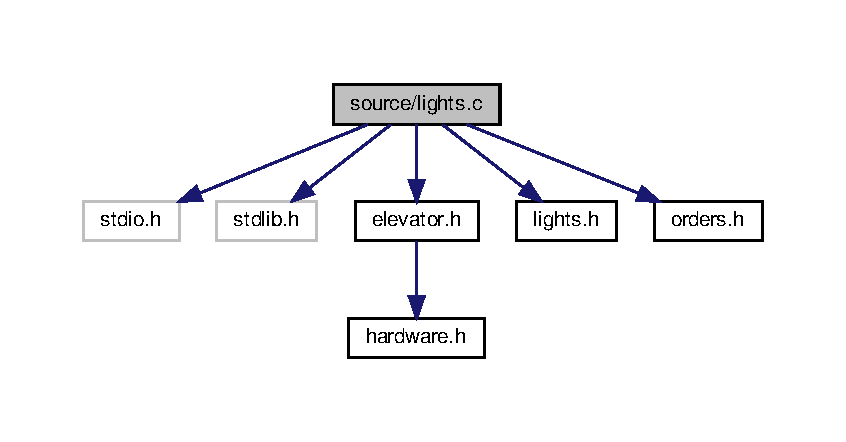
\includegraphics[width=350pt]{lights_8c__incl}
\end{center}
\end{figure}
\subsection*{Functions}
\begin{DoxyCompactItemize}
\item 
void \hyperlink{lights_8c_a2863a72da263e664b63c81d3492fc501}{set\+\_\+order\+\_\+lights\+\_\+up} ()
\begin{DoxyCompactList}\small\item\em Enables the lights for the order up buttons if order up buttons are pressed. \end{DoxyCompactList}\item 
void \hyperlink{lights_8c_ad8a5a5bf8f04d57489b8b48faf47e472}{clear\+\_\+order\+\_\+lights\+\_\+up} ()
\begin{DoxyCompactList}\small\item\em Disables the lights for the order up buttons depending on the existing orders in elevator\+\_\+queue\+\_\+array. \end{DoxyCompactList}\item 
void \hyperlink{lights_8c_a15a04701b6426810d8cd2341c31ffe82}{set\+\_\+order\+\_\+lights\+\_\+down} ()
\begin{DoxyCompactList}\small\item\em Enables the lights for the order down buttons if order down buttons are pressed. \end{DoxyCompactList}\item 
void \hyperlink{lights_8c_aa327ce0cb429b9496dc4545dd6334132}{clear\+\_\+order\+\_\+lights\+\_\+down} ()
\begin{DoxyCompactList}\small\item\em Disables the lights for the order down buttons depending on the existing orders in elevator\+\_\+queue\+\_\+array. \end{DoxyCompactList}\item 
void \hyperlink{lights_8c_a59a579d4f0e661599247b504123b0107}{set\+\_\+order\+\_\+lights\+\_\+inside} ()
\begin{DoxyCompactList}\small\item\em Enables the lights for the cab order buttons if cab order buttons are pressed. \end{DoxyCompactList}\item 
void \hyperlink{lights_8c_a2a9a3a5f2e7f7d944a784026bb138659}{clear\+\_\+order\+\_\+lights\+\_\+inside} ()
\begin{DoxyCompactList}\small\item\em Disables the lights for the cab order buttons depending on the existing orders in elevator\+\_\+queue\+\_\+array. \end{DoxyCompactList}\item 
void \hyperlink{lights_8c_a1636dcf5e18fde0e1f606fe100351854}{set\+\_\+stop\+\_\+light} ()
\begin{DoxyCompactList}\small\item\em Sets the stop light if the stop button is pressed. Disables otherwise. \end{DoxyCompactList}\item 
void \hyperlink{lights_8c_a3d4332abdcc6047bd872881f1ff49d3b}{set\+\_\+floor\+\_\+lights} ()
\begin{DoxyCompactList}\small\item\em Sets the floor light to the last floor the elevator passed. \end{DoxyCompactList}\item 
void \hyperlink{lights_8c_aa7fd7e682d5949fc6a252c239287d4df}{handle\+\_\+lights} ()
\begin{DoxyCompactList}\small\item\em Enables and disables all the elevator lights. \end{DoxyCompactList}\end{DoxyCompactItemize}


\subsection{Function Documentation}
\mbox{\Hypertarget{lights_8c_aa327ce0cb429b9496dc4545dd6334132}\label{lights_8c_aa327ce0cb429b9496dc4545dd6334132}} 
\index{lights.\+c@{lights.\+c}!clear\+\_\+order\+\_\+lights\+\_\+down@{clear\+\_\+order\+\_\+lights\+\_\+down}}
\index{clear\+\_\+order\+\_\+lights\+\_\+down@{clear\+\_\+order\+\_\+lights\+\_\+down}!lights.\+c@{lights.\+c}}
\subsubsection{\texorpdfstring{clear\+\_\+order\+\_\+lights\+\_\+down()}{clear\_order\_lights\_down()}}
{\footnotesize\ttfamily void clear\+\_\+order\+\_\+lights\+\_\+down (\begin{DoxyParamCaption}{ }\end{DoxyParamCaption})}



Disables the lights for the order down buttons depending on the existing orders in elevator\+\_\+queue\+\_\+array. 



Definition at line 32 of file lights.\+c.

\mbox{\Hypertarget{lights_8c_a2a9a3a5f2e7f7d944a784026bb138659}\label{lights_8c_a2a9a3a5f2e7f7d944a784026bb138659}} 
\index{lights.\+c@{lights.\+c}!clear\+\_\+order\+\_\+lights\+\_\+inside@{clear\+\_\+order\+\_\+lights\+\_\+inside}}
\index{clear\+\_\+order\+\_\+lights\+\_\+inside@{clear\+\_\+order\+\_\+lights\+\_\+inside}!lights.\+c@{lights.\+c}}
\subsubsection{\texorpdfstring{clear\+\_\+order\+\_\+lights\+\_\+inside()}{clear\_order\_lights\_inside()}}
{\footnotesize\ttfamily void clear\+\_\+order\+\_\+lights\+\_\+inside (\begin{DoxyParamCaption}{ }\end{DoxyParamCaption})}



Disables the lights for the cab order buttons depending on the existing orders in elevator\+\_\+queue\+\_\+array. 



Definition at line 48 of file lights.\+c.

\mbox{\Hypertarget{lights_8c_ad8a5a5bf8f04d57489b8b48faf47e472}\label{lights_8c_ad8a5a5bf8f04d57489b8b48faf47e472}} 
\index{lights.\+c@{lights.\+c}!clear\+\_\+order\+\_\+lights\+\_\+up@{clear\+\_\+order\+\_\+lights\+\_\+up}}
\index{clear\+\_\+order\+\_\+lights\+\_\+up@{clear\+\_\+order\+\_\+lights\+\_\+up}!lights.\+c@{lights.\+c}}
\subsubsection{\texorpdfstring{clear\+\_\+order\+\_\+lights\+\_\+up()}{clear\_order\_lights\_up()}}
{\footnotesize\ttfamily void clear\+\_\+order\+\_\+lights\+\_\+up (\begin{DoxyParamCaption}{ }\end{DoxyParamCaption})}



Disables the lights for the order up buttons depending on the existing orders in elevator\+\_\+queue\+\_\+array. 



Definition at line 16 of file lights.\+c.

\mbox{\Hypertarget{lights_8c_aa7fd7e682d5949fc6a252c239287d4df}\label{lights_8c_aa7fd7e682d5949fc6a252c239287d4df}} 
\index{lights.\+c@{lights.\+c}!handle\+\_\+lights@{handle\+\_\+lights}}
\index{handle\+\_\+lights@{handle\+\_\+lights}!lights.\+c@{lights.\+c}}
\subsubsection{\texorpdfstring{handle\+\_\+lights()}{handle\_lights()}}
{\footnotesize\ttfamily void handle\+\_\+lights (\begin{DoxyParamCaption}{ }\end{DoxyParamCaption})}



Enables and disables all the elevator lights. 



Definition at line 68 of file lights.\+c.

\mbox{\Hypertarget{lights_8c_a3d4332abdcc6047bd872881f1ff49d3b}\label{lights_8c_a3d4332abdcc6047bd872881f1ff49d3b}} 
\index{lights.\+c@{lights.\+c}!set\+\_\+floor\+\_\+lights@{set\+\_\+floor\+\_\+lights}}
\index{set\+\_\+floor\+\_\+lights@{set\+\_\+floor\+\_\+lights}!lights.\+c@{lights.\+c}}
\subsubsection{\texorpdfstring{set\+\_\+floor\+\_\+lights()}{set\_floor\_lights()}}
{\footnotesize\ttfamily void set\+\_\+floor\+\_\+lights (\begin{DoxyParamCaption}{ }\end{DoxyParamCaption})}



Sets the floor light to the last floor the elevator passed. 



Definition at line 63 of file lights.\+c.

\mbox{\Hypertarget{lights_8c_a15a04701b6426810d8cd2341c31ffe82}\label{lights_8c_a15a04701b6426810d8cd2341c31ffe82}} 
\index{lights.\+c@{lights.\+c}!set\+\_\+order\+\_\+lights\+\_\+down@{set\+\_\+order\+\_\+lights\+\_\+down}}
\index{set\+\_\+order\+\_\+lights\+\_\+down@{set\+\_\+order\+\_\+lights\+\_\+down}!lights.\+c@{lights.\+c}}
\subsubsection{\texorpdfstring{set\+\_\+order\+\_\+lights\+\_\+down()}{set\_order\_lights\_down()}}
{\footnotesize\ttfamily void set\+\_\+order\+\_\+lights\+\_\+down (\begin{DoxyParamCaption}{ }\end{DoxyParamCaption})}



Enables the lights for the order down buttons if order down buttons are pressed. 



Definition at line 24 of file lights.\+c.

\mbox{\Hypertarget{lights_8c_a59a579d4f0e661599247b504123b0107}\label{lights_8c_a59a579d4f0e661599247b504123b0107}} 
\index{lights.\+c@{lights.\+c}!set\+\_\+order\+\_\+lights\+\_\+inside@{set\+\_\+order\+\_\+lights\+\_\+inside}}
\index{set\+\_\+order\+\_\+lights\+\_\+inside@{set\+\_\+order\+\_\+lights\+\_\+inside}!lights.\+c@{lights.\+c}}
\subsubsection{\texorpdfstring{set\+\_\+order\+\_\+lights\+\_\+inside()}{set\_order\_lights\_inside()}}
{\footnotesize\ttfamily void set\+\_\+order\+\_\+lights\+\_\+inside (\begin{DoxyParamCaption}{ }\end{DoxyParamCaption})}



Enables the lights for the cab order buttons if cab order buttons are pressed. 



Definition at line 40 of file lights.\+c.

\mbox{\Hypertarget{lights_8c_a2863a72da263e664b63c81d3492fc501}\label{lights_8c_a2863a72da263e664b63c81d3492fc501}} 
\index{lights.\+c@{lights.\+c}!set\+\_\+order\+\_\+lights\+\_\+up@{set\+\_\+order\+\_\+lights\+\_\+up}}
\index{set\+\_\+order\+\_\+lights\+\_\+up@{set\+\_\+order\+\_\+lights\+\_\+up}!lights.\+c@{lights.\+c}}
\subsubsection{\texorpdfstring{set\+\_\+order\+\_\+lights\+\_\+up()}{set\_order\_lights\_up()}}
{\footnotesize\ttfamily void set\+\_\+order\+\_\+lights\+\_\+up (\begin{DoxyParamCaption}{ }\end{DoxyParamCaption})}



Enables the lights for the order up buttons if order up buttons are pressed. 



Definition at line 8 of file lights.\+c.

\mbox{\Hypertarget{lights_8c_a1636dcf5e18fde0e1f606fe100351854}\label{lights_8c_a1636dcf5e18fde0e1f606fe100351854}} 
\index{lights.\+c@{lights.\+c}!set\+\_\+stop\+\_\+light@{set\+\_\+stop\+\_\+light}}
\index{set\+\_\+stop\+\_\+light@{set\+\_\+stop\+\_\+light}!lights.\+c@{lights.\+c}}
\subsubsection{\texorpdfstring{set\+\_\+stop\+\_\+light()}{set\_stop\_light()}}
{\footnotesize\ttfamily void set\+\_\+stop\+\_\+light (\begin{DoxyParamCaption}{ }\end{DoxyParamCaption})}



Sets the stop light if the stop button is pressed. Disables otherwise. 



Definition at line 56 of file lights.\+c.


\hypertarget{lights_8h}{}\section{source/lights.h File Reference}
\label{lights_8h}\index{source/lights.\+h@{source/lights.\+h}}


All functions handling the lights.  


This graph shows which files directly or indirectly include this file\+:
\nopagebreak
\begin{figure}[H]
\begin{center}
\leavevmode
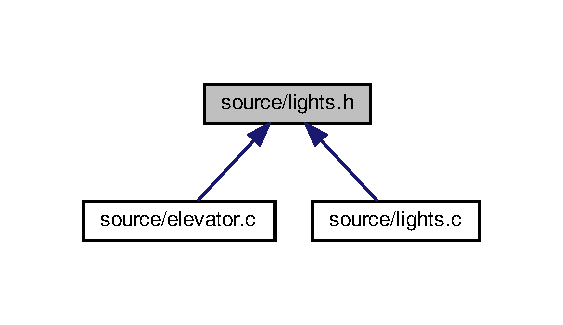
\includegraphics[width=270pt]{lights_8h__dep__incl}
\end{center}
\end{figure}
\subsection*{Functions}
\begin{DoxyCompactItemize}
\item 
void \hyperlink{lights_8h_a2863a72da263e664b63c81d3492fc501}{set\+\_\+order\+\_\+lights\+\_\+up} ()
\begin{DoxyCompactList}\small\item\em Enables the lights for the order up buttons if order up buttons are pressed. \end{DoxyCompactList}\item 
void \hyperlink{lights_8h_ad8a5a5bf8f04d57489b8b48faf47e472}{clear\+\_\+order\+\_\+lights\+\_\+up} ()
\begin{DoxyCompactList}\small\item\em Disables the lights for the order up buttons depending on the existing orders in elevator\+\_\+queue\+\_\+array. \end{DoxyCompactList}\item 
void \hyperlink{lights_8h_a15a04701b6426810d8cd2341c31ffe82}{set\+\_\+order\+\_\+lights\+\_\+down} ()
\begin{DoxyCompactList}\small\item\em Enables the lights for the order down buttons if order down buttons are pressed. \end{DoxyCompactList}\item 
void \hyperlink{lights_8h_aa327ce0cb429b9496dc4545dd6334132}{clear\+\_\+order\+\_\+lights\+\_\+down} ()
\begin{DoxyCompactList}\small\item\em Disables the lights for the order down buttons depending on the existing orders in elevator\+\_\+queue\+\_\+array. \end{DoxyCompactList}\item 
void \hyperlink{lights_8h_a59a579d4f0e661599247b504123b0107}{set\+\_\+order\+\_\+lights\+\_\+inside} ()
\begin{DoxyCompactList}\small\item\em Enables the lights for the cab order buttons if cab order buttons are pressed. \end{DoxyCompactList}\item 
void \hyperlink{lights_8h_a2a9a3a5f2e7f7d944a784026bb138659}{clear\+\_\+order\+\_\+lights\+\_\+inside} ()
\begin{DoxyCompactList}\small\item\em Disables the lights for the cab order buttons depending on the existing orders in elevator\+\_\+queue\+\_\+array. \end{DoxyCompactList}\item 
void \hyperlink{lights_8h_a1636dcf5e18fde0e1f606fe100351854}{set\+\_\+stop\+\_\+light} ()
\begin{DoxyCompactList}\small\item\em Sets the stop light if the stop button is pressed. Disables otherwise. \end{DoxyCompactList}\item 
void \hyperlink{lights_8h_a3d4332abdcc6047bd872881f1ff49d3b}{set\+\_\+floor\+\_\+lights} ()
\begin{DoxyCompactList}\small\item\em Sets the floor light to the last floor the elevator passed. \end{DoxyCompactList}\item 
void \hyperlink{lights_8h_aa7fd7e682d5949fc6a252c239287d4df}{handle\+\_\+lights} ()
\begin{DoxyCompactList}\small\item\em Enables and disables all the elevator lights. \end{DoxyCompactList}\end{DoxyCompactItemize}


\subsection{Detailed Description}
All functions handling the lights. 



\subsection{Function Documentation}
\mbox{\Hypertarget{lights_8h_aa327ce0cb429b9496dc4545dd6334132}\label{lights_8h_aa327ce0cb429b9496dc4545dd6334132}} 
\index{lights.\+h@{lights.\+h}!clear\+\_\+order\+\_\+lights\+\_\+down@{clear\+\_\+order\+\_\+lights\+\_\+down}}
\index{clear\+\_\+order\+\_\+lights\+\_\+down@{clear\+\_\+order\+\_\+lights\+\_\+down}!lights.\+h@{lights.\+h}}
\subsubsection{\texorpdfstring{clear\+\_\+order\+\_\+lights\+\_\+down()}{clear\_order\_lights\_down()}}
{\footnotesize\ttfamily void clear\+\_\+order\+\_\+lights\+\_\+down (\begin{DoxyParamCaption}{ }\end{DoxyParamCaption})}



Disables the lights for the order down buttons depending on the existing orders in elevator\+\_\+queue\+\_\+array. 



Definition at line 32 of file lights.\+c.

\mbox{\Hypertarget{lights_8h_a2a9a3a5f2e7f7d944a784026bb138659}\label{lights_8h_a2a9a3a5f2e7f7d944a784026bb138659}} 
\index{lights.\+h@{lights.\+h}!clear\+\_\+order\+\_\+lights\+\_\+inside@{clear\+\_\+order\+\_\+lights\+\_\+inside}}
\index{clear\+\_\+order\+\_\+lights\+\_\+inside@{clear\+\_\+order\+\_\+lights\+\_\+inside}!lights.\+h@{lights.\+h}}
\subsubsection{\texorpdfstring{clear\+\_\+order\+\_\+lights\+\_\+inside()}{clear\_order\_lights\_inside()}}
{\footnotesize\ttfamily void clear\+\_\+order\+\_\+lights\+\_\+inside (\begin{DoxyParamCaption}{ }\end{DoxyParamCaption})}



Disables the lights for the cab order buttons depending on the existing orders in elevator\+\_\+queue\+\_\+array. 



Definition at line 48 of file lights.\+c.

\mbox{\Hypertarget{lights_8h_ad8a5a5bf8f04d57489b8b48faf47e472}\label{lights_8h_ad8a5a5bf8f04d57489b8b48faf47e472}} 
\index{lights.\+h@{lights.\+h}!clear\+\_\+order\+\_\+lights\+\_\+up@{clear\+\_\+order\+\_\+lights\+\_\+up}}
\index{clear\+\_\+order\+\_\+lights\+\_\+up@{clear\+\_\+order\+\_\+lights\+\_\+up}!lights.\+h@{lights.\+h}}
\subsubsection{\texorpdfstring{clear\+\_\+order\+\_\+lights\+\_\+up()}{clear\_order\_lights\_up()}}
{\footnotesize\ttfamily void clear\+\_\+order\+\_\+lights\+\_\+up (\begin{DoxyParamCaption}{ }\end{DoxyParamCaption})}



Disables the lights for the order up buttons depending on the existing orders in elevator\+\_\+queue\+\_\+array. 



Definition at line 16 of file lights.\+c.

\mbox{\Hypertarget{lights_8h_aa7fd7e682d5949fc6a252c239287d4df}\label{lights_8h_aa7fd7e682d5949fc6a252c239287d4df}} 
\index{lights.\+h@{lights.\+h}!handle\+\_\+lights@{handle\+\_\+lights}}
\index{handle\+\_\+lights@{handle\+\_\+lights}!lights.\+h@{lights.\+h}}
\subsubsection{\texorpdfstring{handle\+\_\+lights()}{handle\_lights()}}
{\footnotesize\ttfamily void handle\+\_\+lights (\begin{DoxyParamCaption}{ }\end{DoxyParamCaption})}



Enables and disables all the elevator lights. 



Definition at line 68 of file lights.\+c.

\mbox{\Hypertarget{lights_8h_a3d4332abdcc6047bd872881f1ff49d3b}\label{lights_8h_a3d4332abdcc6047bd872881f1ff49d3b}} 
\index{lights.\+h@{lights.\+h}!set\+\_\+floor\+\_\+lights@{set\+\_\+floor\+\_\+lights}}
\index{set\+\_\+floor\+\_\+lights@{set\+\_\+floor\+\_\+lights}!lights.\+h@{lights.\+h}}
\subsubsection{\texorpdfstring{set\+\_\+floor\+\_\+lights()}{set\_floor\_lights()}}
{\footnotesize\ttfamily void set\+\_\+floor\+\_\+lights (\begin{DoxyParamCaption}{ }\end{DoxyParamCaption})}



Sets the floor light to the last floor the elevator passed. 



Definition at line 63 of file lights.\+c.

\mbox{\Hypertarget{lights_8h_a15a04701b6426810d8cd2341c31ffe82}\label{lights_8h_a15a04701b6426810d8cd2341c31ffe82}} 
\index{lights.\+h@{lights.\+h}!set\+\_\+order\+\_\+lights\+\_\+down@{set\+\_\+order\+\_\+lights\+\_\+down}}
\index{set\+\_\+order\+\_\+lights\+\_\+down@{set\+\_\+order\+\_\+lights\+\_\+down}!lights.\+h@{lights.\+h}}
\subsubsection{\texorpdfstring{set\+\_\+order\+\_\+lights\+\_\+down()}{set\_order\_lights\_down()}}
{\footnotesize\ttfamily void set\+\_\+order\+\_\+lights\+\_\+down (\begin{DoxyParamCaption}{ }\end{DoxyParamCaption})}



Enables the lights for the order down buttons if order down buttons are pressed. 



Definition at line 24 of file lights.\+c.

\mbox{\Hypertarget{lights_8h_a59a579d4f0e661599247b504123b0107}\label{lights_8h_a59a579d4f0e661599247b504123b0107}} 
\index{lights.\+h@{lights.\+h}!set\+\_\+order\+\_\+lights\+\_\+inside@{set\+\_\+order\+\_\+lights\+\_\+inside}}
\index{set\+\_\+order\+\_\+lights\+\_\+inside@{set\+\_\+order\+\_\+lights\+\_\+inside}!lights.\+h@{lights.\+h}}
\subsubsection{\texorpdfstring{set\+\_\+order\+\_\+lights\+\_\+inside()}{set\_order\_lights\_inside()}}
{\footnotesize\ttfamily void set\+\_\+order\+\_\+lights\+\_\+inside (\begin{DoxyParamCaption}{ }\end{DoxyParamCaption})}



Enables the lights for the cab order buttons if cab order buttons are pressed. 



Definition at line 40 of file lights.\+c.

\mbox{\Hypertarget{lights_8h_a2863a72da263e664b63c81d3492fc501}\label{lights_8h_a2863a72da263e664b63c81d3492fc501}} 
\index{lights.\+h@{lights.\+h}!set\+\_\+order\+\_\+lights\+\_\+up@{set\+\_\+order\+\_\+lights\+\_\+up}}
\index{set\+\_\+order\+\_\+lights\+\_\+up@{set\+\_\+order\+\_\+lights\+\_\+up}!lights.\+h@{lights.\+h}}
\subsubsection{\texorpdfstring{set\+\_\+order\+\_\+lights\+\_\+up()}{set\_order\_lights\_up()}}
{\footnotesize\ttfamily void set\+\_\+order\+\_\+lights\+\_\+up (\begin{DoxyParamCaption}{ }\end{DoxyParamCaption})}



Enables the lights for the order up buttons if order up buttons are pressed. 



Definition at line 8 of file lights.\+c.

\mbox{\Hypertarget{lights_8h_a1636dcf5e18fde0e1f606fe100351854}\label{lights_8h_a1636dcf5e18fde0e1f606fe100351854}} 
\index{lights.\+h@{lights.\+h}!set\+\_\+stop\+\_\+light@{set\+\_\+stop\+\_\+light}}
\index{set\+\_\+stop\+\_\+light@{set\+\_\+stop\+\_\+light}!lights.\+h@{lights.\+h}}
\subsubsection{\texorpdfstring{set\+\_\+stop\+\_\+light()}{set\_stop\_light()}}
{\footnotesize\ttfamily void set\+\_\+stop\+\_\+light (\begin{DoxyParamCaption}{ }\end{DoxyParamCaption})}



Sets the stop light if the stop button is pressed. Disables otherwise. 



Definition at line 56 of file lights.\+c.


\hypertarget{main_8c}{}\section{source/main.c File Reference}
\label{main_8c}\index{source/main.\+c@{source/main.\+c}}
{\ttfamily \#include $<$stdio.\+h$>$}\newline
{\ttfamily \#include $<$stdlib.\+h$>$}\newline
{\ttfamily \#include \char`\"{}elevator.\+h\char`\"{}}\newline
{\ttfamily \#include \char`\"{}signal.\+h\char`\"{}}\newline
Include dependency graph for main.\+c\+:\nopagebreak
\begin{figure}[H]
\begin{center}
\leavevmode
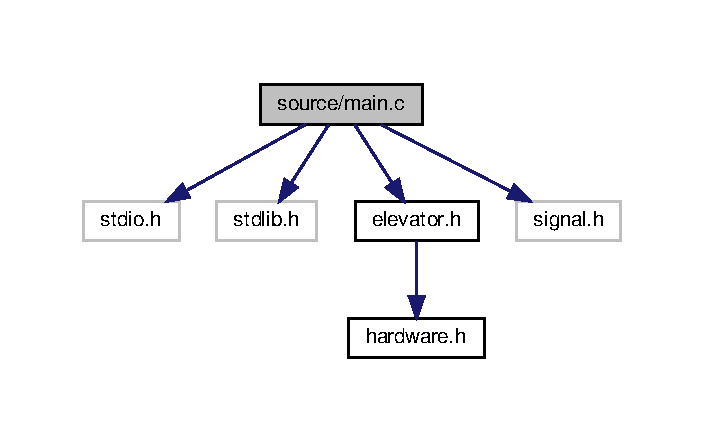
\includegraphics[width=338pt]{main_8c__incl}
\end{center}
\end{figure}
\subsection*{Functions}
\begin{DoxyCompactItemize}
\item 
int \hyperlink{main_8c_ae66f6b31b5ad750f1fe042a706a4e3d4}{main} ()
\end{DoxyCompactItemize}


\subsection{Function Documentation}
\mbox{\Hypertarget{main_8c_ae66f6b31b5ad750f1fe042a706a4e3d4}\label{main_8c_ae66f6b31b5ad750f1fe042a706a4e3d4}} 
\index{main.\+c@{main.\+c}!main@{main}}
\index{main@{main}!main.\+c@{main.\+c}}
\subsubsection{\texorpdfstring{main()}{main()}}
{\footnotesize\ttfamily int main (\begin{DoxyParamCaption}{ }\end{DoxyParamCaption})}



Definition at line 13 of file main.\+c.


\hypertarget{orders_8c}{}\section{source/orders.c File Reference}
\label{orders_8c}\index{source/orders.\+c@{source/orders.\+c}}
{\ttfamily \#include $<$stdio.\+h$>$}\newline
{\ttfamily \#include $<$stdlib.\+h$>$}\newline
{\ttfamily \#include \char`\"{}elevator.\+h\char`\"{}}\newline
{\ttfamily \#include \char`\"{}orders.\+h\char`\"{}}\newline
Include dependency graph for orders.\+c\+:
\nopagebreak
\begin{figure}[H]
\begin{center}
\leavevmode
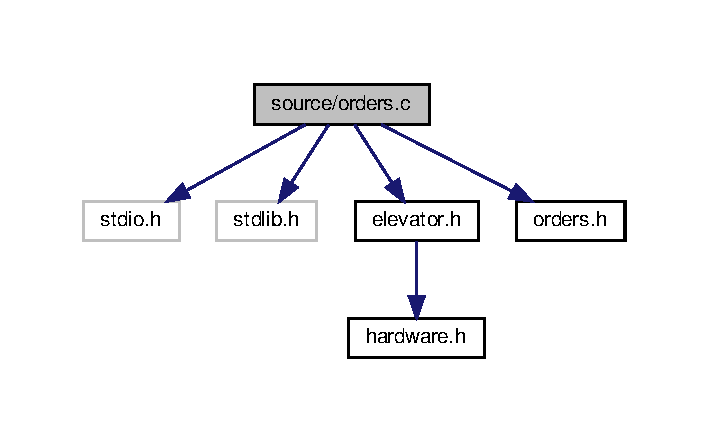
\includegraphics[width=340pt]{orders_8c__incl}
\end{center}
\end{figure}
\subsection*{Functions}
\begin{DoxyCompactItemize}
\item 
int \hyperlink{orders_8c_ac426009b9dd5bd9bc76949a454a320a6}{get\+\_\+current\+\_\+direction} ()
\begin{DoxyCompactList}\small\item\em Gets the current direction. \end{DoxyCompactList}\item 
void \hyperlink{orders_8c_acf6f3f01ccc5d2cc5678499e4a992400}{set\+\_\+current\+\_\+direction} (int direction)
\begin{DoxyCompactList}\small\item\em Sets current\+\_\+direction to {\ttfamily direction} . \end{DoxyCompactList}\item 
int \hyperlink{orders_8c_acf20a30f171233e040ea4b4b2e5f4a46}{get\+\_\+order\+\_\+at\+\_\+floor} (int floor)
\begin{DoxyCompactList}\small\item\em Gets the value of elevator\+\_\+order\+\_\+array with index {\ttfamily floor} . \end{DoxyCompactList}\item 
void \hyperlink{orders_8c_ac6cd7c279c95b7a210719dffada982d8}{set\+\_\+order\+\_\+at\+\_\+floor} (int floor, int order)
\begin{DoxyCompactList}\small\item\em Sets the value of elevator\+\_\+order\+\_\+array with index {\ttfamily floor} to {\ttfamily order} . \end{DoxyCompactList}\item 
void \hyperlink{orders_8c_ae53d74727711dab412fb4c01aaa029da}{set\+\_\+order\+\_\+up} ()
\begin{DoxyCompactList}\small\item\em Updates elevator\+\_\+order\+\_\+array if any of the order up buttons are pressed. \end{DoxyCompactList}\item 
void \hyperlink{orders_8c_a4cf3627d1c6a40e9af29458da858558b}{set\+\_\+order\+\_\+down} ()
\begin{DoxyCompactList}\small\item\em Updates elevator\+\_\+order\+\_\+array if any of the order down buttons are pressed. \end{DoxyCompactList}\item 
void \hyperlink{orders_8c_ad81206d15e03830095bf5012a7ec48e0}{set\+\_\+order\+\_\+inside} ()
\begin{DoxyCompactList}\small\item\em Updates elevator\+\_\+order\+\_\+array if any of the order inside buttons are pressed. \end{DoxyCompactList}\item 
void \hyperlink{orders_8c_a60ab7f01650e26035d6ed4c623d3659d}{handle\+\_\+orders} ()
\begin{DoxyCompactList}\small\item\em Updates elevator\+\_\+order\+\_\+array if any order buttons are pressed. \end{DoxyCompactList}\item 
int \hyperlink{orders_8c_ae1f8082a7b2f16cecfd3ace6d8c6d73f}{check\+\_\+orders\+\_\+above} (int starting\+\_\+point)
\begin{DoxyCompactList}\small\item\em Checks if there are any order above {\ttfamily starting\+\_\+point} . \end{DoxyCompactList}\item 
int \hyperlink{orders_8c_a46e249c28b02726e1867ae718644a33f}{check\+\_\+orders\+\_\+below} (int starting\+\_\+point)
\begin{DoxyCompactList}\small\item\em Checks if there are any order below {\ttfamily starting\+\_\+point} . \end{DoxyCompactList}\item 
int \hyperlink{orders_8c_a5a309ac4f781a8b05b200d09a16987dc}{get\+\_\+order\+\_\+count} ()
\begin{DoxyCompactList}\small\item\em Gets the total amount of unattended orders. \end{DoxyCompactList}\item 
void \hyperlink{orders_8c_a1ae3ab02b290c9ba95abb9a3fc5bdbd1}{update\+\_\+current\+\_\+direction} ()
\begin{DoxyCompactList}\small\item\em Updates current\+\_\+direction based on existing orders, current\+\_\+direction and last\+\_\+direction. \end{DoxyCompactList}\item 
int \hyperlink{orders_8c_a263178a16b07955e026ff65f9f246d60}{check\+\_\+up\+\_\+at\+\_\+floor} ()
\begin{DoxyCompactList}\small\item\em Checks if there are any up orders at the current floor. \end{DoxyCompactList}\item 
int \hyperlink{orders_8c_a6a754d33f3fb49024aea10f590f25dea}{check\+\_\+down\+\_\+at\+\_\+floor} ()
\begin{DoxyCompactList}\small\item\em Checks if there are any down orders at the current floor. \end{DoxyCompactList}\item 
int \hyperlink{orders_8c_aa2814fca8943e13c07a75aca10cc4517}{check\+\_\+both\+\_\+or\+\_\+cab\+\_\+at\+\_\+floor} ()
\begin{DoxyCompactList}\small\item\em Checks if there are any cab orders or up and down orders simultaneously at the current floor. \end{DoxyCompactList}\item 
int \hyperlink{orders_8c_a0be2dc6cef3d1e0ebcc153b9b0f78d93}{check\+\_\+arrival} ()
\begin{DoxyCompactList}\small\item\em Checks if the elevator has arrived at a floor with an order that needs to be attended. \end{DoxyCompactList}\item 
void \hyperlink{orders_8c_a6206e5203639ca23d84820e2ffb108a3}{clear\+\_\+all\+\_\+orders} ()
\begin{DoxyCompactList}\small\item\em Clears all existing orders in elevator\+\_\+order\+\_\+array. \end{DoxyCompactList}\item 
void \hyperlink{orders_8c_a246f5cd101e20bda3d5f2607f8e56f0c}{print\+\_\+all\+\_\+orders} ()
\begin{DoxyCompactList}\small\item\em Prints all existing orders in elevator\+\_\+order\+\_\+array. \end{DoxyCompactList}\item 
int \hyperlink{orders_8c_a47efe536e1dd0d64e2f4edf1af2345b4}{bool\+\_\+order\+\_\+at\+\_\+floor} (int floor)
\begin{DoxyCompactList}\small\item\em Checks if there are any orders at at {\ttfamily floor} . \end{DoxyCompactList}\end{DoxyCompactItemize}
\subsection*{Variables}
\begin{DoxyCompactItemize}
\item 
int \hyperlink{orders_8c_aafffa54a4465b20eac09db2c47fa54e2}{direction\+\_\+from\+\_\+last\+\_\+floor}
\item 
int \hyperlink{orders_8c_a6ca3ab5487e8be51322670cf9c3d8d1f}{elevator\+\_\+order\+\_\+array} \mbox{[}4\mbox{]}
\end{DoxyCompactItemize}


\subsection{Function Documentation}
\mbox{\Hypertarget{orders_8c_a47efe536e1dd0d64e2f4edf1af2345b4}\label{orders_8c_a47efe536e1dd0d64e2f4edf1af2345b4}} 
\index{orders.\+c@{orders.\+c}!bool\+\_\+order\+\_\+at\+\_\+floor@{bool\+\_\+order\+\_\+at\+\_\+floor}}
\index{bool\+\_\+order\+\_\+at\+\_\+floor@{bool\+\_\+order\+\_\+at\+\_\+floor}!orders.\+c@{orders.\+c}}
\subsubsection{\texorpdfstring{bool\+\_\+order\+\_\+at\+\_\+floor()}{bool\_order\_at\_floor()}}
{\footnotesize\ttfamily int bool\+\_\+order\+\_\+at\+\_\+floor (\begin{DoxyParamCaption}\item[{int}]{floor }\end{DoxyParamCaption})}



Checks if there are any orders at at {\ttfamily floor} . 


\begin{DoxyParams}{Parameters}
{\em floor} & \\
\hline
\end{DoxyParams}
\begin{DoxyReturn}{Returns}
Return 1 if order at requested floor. Return 0 otherwise. 
\end{DoxyReturn}


Definition at line 185 of file orders.\+c.

\mbox{\Hypertarget{orders_8c_a0be2dc6cef3d1e0ebcc153b9b0f78d93}\label{orders_8c_a0be2dc6cef3d1e0ebcc153b9b0f78d93}} 
\index{orders.\+c@{orders.\+c}!check\+\_\+arrival@{check\+\_\+arrival}}
\index{check\+\_\+arrival@{check\+\_\+arrival}!orders.\+c@{orders.\+c}}
\subsubsection{\texorpdfstring{check\+\_\+arrival()}{check\_arrival()}}
{\footnotesize\ttfamily int check\+\_\+arrival (\begin{DoxyParamCaption}{ }\end{DoxyParamCaption})}



Checks if the elevator has arrived at a floor with an order that needs to be attended. 

\begin{DoxyReturn}{Returns}
Return 1 if arrived at floor with order. Return 0 otherwise. 
\end{DoxyReturn}


Definition at line 154 of file orders.\+c.

\mbox{\Hypertarget{orders_8c_aa2814fca8943e13c07a75aca10cc4517}\label{orders_8c_aa2814fca8943e13c07a75aca10cc4517}} 
\index{orders.\+c@{orders.\+c}!check\+\_\+both\+\_\+or\+\_\+cab\+\_\+at\+\_\+floor@{check\+\_\+both\+\_\+or\+\_\+cab\+\_\+at\+\_\+floor}}
\index{check\+\_\+both\+\_\+or\+\_\+cab\+\_\+at\+\_\+floor@{check\+\_\+both\+\_\+or\+\_\+cab\+\_\+at\+\_\+floor}!orders.\+c@{orders.\+c}}
\subsubsection{\texorpdfstring{check\+\_\+both\+\_\+or\+\_\+cab\+\_\+at\+\_\+floor()}{check\_both\_or\_cab\_at\_floor()}}
{\footnotesize\ttfamily int check\+\_\+both\+\_\+or\+\_\+cab\+\_\+at\+\_\+floor (\begin{DoxyParamCaption}{ }\end{DoxyParamCaption})}



Checks if there are any cab orders or up and down orders simultaneously at the current floor. 

\begin{DoxyReturn}{Returns}
Return 1 if cab order or up and down order at floor. Return 0 otherwise. 
\end{DoxyReturn}


Definition at line 145 of file orders.\+c.

\mbox{\Hypertarget{orders_8c_a6a754d33f3fb49024aea10f590f25dea}\label{orders_8c_a6a754d33f3fb49024aea10f590f25dea}} 
\index{orders.\+c@{orders.\+c}!check\+\_\+down\+\_\+at\+\_\+floor@{check\+\_\+down\+\_\+at\+\_\+floor}}
\index{check\+\_\+down\+\_\+at\+\_\+floor@{check\+\_\+down\+\_\+at\+\_\+floor}!orders.\+c@{orders.\+c}}
\subsubsection{\texorpdfstring{check\+\_\+down\+\_\+at\+\_\+floor()}{check\_down\_at\_floor()}}
{\footnotesize\ttfamily int check\+\_\+down\+\_\+at\+\_\+floor (\begin{DoxyParamCaption}{ }\end{DoxyParamCaption})}



Checks if there are any down orders at the current floor. 

\begin{DoxyReturn}{Returns}
Return 1 if down order at floor. Return 0 otherwise. 
\end{DoxyReturn}


Definition at line 136 of file orders.\+c.

\mbox{\Hypertarget{orders_8c_ae1f8082a7b2f16cecfd3ace6d8c6d73f}\label{orders_8c_ae1f8082a7b2f16cecfd3ace6d8c6d73f}} 
\index{orders.\+c@{orders.\+c}!check\+\_\+orders\+\_\+above@{check\+\_\+orders\+\_\+above}}
\index{check\+\_\+orders\+\_\+above@{check\+\_\+orders\+\_\+above}!orders.\+c@{orders.\+c}}
\subsubsection{\texorpdfstring{check\+\_\+orders\+\_\+above()}{check\_orders\_above()}}
{\footnotesize\ttfamily int check\+\_\+orders\+\_\+above (\begin{DoxyParamCaption}\item[{int}]{starting\+\_\+point }\end{DoxyParamCaption})}



Checks if there are any order above {\ttfamily starting\+\_\+point} . 


\begin{DoxyParams}{Parameters}
{\em starting\+\_\+point} & \\
\hline
\end{DoxyParams}
\begin{DoxyReturn}{Returns}
Return 1 if there are orders above. Return 0 otherwise. 
\end{DoxyReturn}


Definition at line 70 of file orders.\+c.

\mbox{\Hypertarget{orders_8c_a46e249c28b02726e1867ae718644a33f}\label{orders_8c_a46e249c28b02726e1867ae718644a33f}} 
\index{orders.\+c@{orders.\+c}!check\+\_\+orders\+\_\+below@{check\+\_\+orders\+\_\+below}}
\index{check\+\_\+orders\+\_\+below@{check\+\_\+orders\+\_\+below}!orders.\+c@{orders.\+c}}
\subsubsection{\texorpdfstring{check\+\_\+orders\+\_\+below()}{check\_orders\_below()}}
{\footnotesize\ttfamily int check\+\_\+orders\+\_\+below (\begin{DoxyParamCaption}\item[{int}]{starting\+\_\+point }\end{DoxyParamCaption})}



Checks if there are any order below {\ttfamily starting\+\_\+point} . 


\begin{DoxyParams}{Parameters}
{\em starting\+\_\+point} & \\
\hline
\end{DoxyParams}
\begin{DoxyReturn}{Returns}
Return 1 if there are orders below. Return 0 otherwise. 
\end{DoxyReturn}


Definition at line 81 of file orders.\+c.

\mbox{\Hypertarget{orders_8c_a263178a16b07955e026ff65f9f246d60}\label{orders_8c_a263178a16b07955e026ff65f9f246d60}} 
\index{orders.\+c@{orders.\+c}!check\+\_\+up\+\_\+at\+\_\+floor@{check\+\_\+up\+\_\+at\+\_\+floor}}
\index{check\+\_\+up\+\_\+at\+\_\+floor@{check\+\_\+up\+\_\+at\+\_\+floor}!orders.\+c@{orders.\+c}}
\subsubsection{\texorpdfstring{check\+\_\+up\+\_\+at\+\_\+floor()}{check\_up\_at\_floor()}}
{\footnotesize\ttfamily int check\+\_\+up\+\_\+at\+\_\+floor (\begin{DoxyParamCaption}{ }\end{DoxyParamCaption})}



Checks if there are any up orders at the current floor. 

\begin{DoxyReturn}{Returns}
Return 1 if up order at floor. Return 0 otherwise. 
\end{DoxyReturn}


Definition at line 127 of file orders.\+c.

\mbox{\Hypertarget{orders_8c_a6206e5203639ca23d84820e2ffb108a3}\label{orders_8c_a6206e5203639ca23d84820e2ffb108a3}} 
\index{orders.\+c@{orders.\+c}!clear\+\_\+all\+\_\+orders@{clear\+\_\+all\+\_\+orders}}
\index{clear\+\_\+all\+\_\+orders@{clear\+\_\+all\+\_\+orders}!orders.\+c@{orders.\+c}}
\subsubsection{\texorpdfstring{clear\+\_\+all\+\_\+orders()}{clear\_all\_orders()}}
{\footnotesize\ttfamily void clear\+\_\+all\+\_\+orders (\begin{DoxyParamCaption}{ }\end{DoxyParamCaption})}



Clears all existing orders in elevator\+\_\+order\+\_\+array. 



Definition at line 173 of file orders.\+c.

\mbox{\Hypertarget{orders_8c_ac426009b9dd5bd9bc76949a454a320a6}\label{orders_8c_ac426009b9dd5bd9bc76949a454a320a6}} 
\index{orders.\+c@{orders.\+c}!get\+\_\+current\+\_\+direction@{get\+\_\+current\+\_\+direction}}
\index{get\+\_\+current\+\_\+direction@{get\+\_\+current\+\_\+direction}!orders.\+c@{orders.\+c}}
\subsubsection{\texorpdfstring{get\+\_\+current\+\_\+direction()}{get\_current\_direction()}}
{\footnotesize\ttfamily int get\+\_\+current\+\_\+direction (\begin{DoxyParamCaption}{ }\end{DoxyParamCaption})}



Gets the current direction. 

\begin{DoxyReturn}{Returns}
Return current\+\_\+direction. 
\end{DoxyReturn}


Definition at line 13 of file orders.\+c.

\mbox{\Hypertarget{orders_8c_acf20a30f171233e040ea4b4b2e5f4a46}\label{orders_8c_acf20a30f171233e040ea4b4b2e5f4a46}} 
\index{orders.\+c@{orders.\+c}!get\+\_\+order\+\_\+at\+\_\+floor@{get\+\_\+order\+\_\+at\+\_\+floor}}
\index{get\+\_\+order\+\_\+at\+\_\+floor@{get\+\_\+order\+\_\+at\+\_\+floor}!orders.\+c@{orders.\+c}}
\subsubsection{\texorpdfstring{get\+\_\+order\+\_\+at\+\_\+floor()}{get\_order\_at\_floor()}}
{\footnotesize\ttfamily int get\+\_\+order\+\_\+at\+\_\+floor (\begin{DoxyParamCaption}\item[{int}]{floor }\end{DoxyParamCaption})}



Gets the value of elevator\+\_\+order\+\_\+array with index {\ttfamily floor} . 


\begin{DoxyParams}{Parameters}
{\em floor} & \\
\hline
\end{DoxyParams}
\begin{DoxyReturn}{Returns}
Return the value of elevator\+\_\+order\+\_\+array with selected index. 
\end{DoxyReturn}


Definition at line 21 of file orders.\+c.

\mbox{\Hypertarget{orders_8c_a5a309ac4f781a8b05b200d09a16987dc}\label{orders_8c_a5a309ac4f781a8b05b200d09a16987dc}} 
\index{orders.\+c@{orders.\+c}!get\+\_\+order\+\_\+count@{get\+\_\+order\+\_\+count}}
\index{get\+\_\+order\+\_\+count@{get\+\_\+order\+\_\+count}!orders.\+c@{orders.\+c}}
\subsubsection{\texorpdfstring{get\+\_\+order\+\_\+count()}{get\_order\_count()}}
{\footnotesize\ttfamily int get\+\_\+order\+\_\+count (\begin{DoxyParamCaption}{ }\end{DoxyParamCaption})}



Gets the total amount of unattended orders. 

\begin{DoxyReturn}{Returns}
Return the total amount of unattended orders. 
\end{DoxyReturn}


Definition at line 92 of file orders.\+c.

\mbox{\Hypertarget{orders_8c_a60ab7f01650e26035d6ed4c623d3659d}\label{orders_8c_a60ab7f01650e26035d6ed4c623d3659d}} 
\index{orders.\+c@{orders.\+c}!handle\+\_\+orders@{handle\+\_\+orders}}
\index{handle\+\_\+orders@{handle\+\_\+orders}!orders.\+c@{orders.\+c}}
\subsubsection{\texorpdfstring{handle\+\_\+orders()}{handle\_orders()}}
{\footnotesize\ttfamily void handle\+\_\+orders (\begin{DoxyParamCaption}{ }\end{DoxyParamCaption})}



Updates elevator\+\_\+order\+\_\+array if any order buttons are pressed. 



Definition at line 64 of file orders.\+c.

\mbox{\Hypertarget{orders_8c_a246f5cd101e20bda3d5f2607f8e56f0c}\label{orders_8c_a246f5cd101e20bda3d5f2607f8e56f0c}} 
\index{orders.\+c@{orders.\+c}!print\+\_\+all\+\_\+orders@{print\+\_\+all\+\_\+orders}}
\index{print\+\_\+all\+\_\+orders@{print\+\_\+all\+\_\+orders}!orders.\+c@{orders.\+c}}
\subsubsection{\texorpdfstring{print\+\_\+all\+\_\+orders()}{print\_all\_orders()}}
{\footnotesize\ttfamily void print\+\_\+all\+\_\+orders (\begin{DoxyParamCaption}{ }\end{DoxyParamCaption})}



Prints all existing orders in elevator\+\_\+order\+\_\+array. 



Definition at line 179 of file orders.\+c.

\mbox{\Hypertarget{orders_8c_acf6f3f01ccc5d2cc5678499e4a992400}\label{orders_8c_acf6f3f01ccc5d2cc5678499e4a992400}} 
\index{orders.\+c@{orders.\+c}!set\+\_\+current\+\_\+direction@{set\+\_\+current\+\_\+direction}}
\index{set\+\_\+current\+\_\+direction@{set\+\_\+current\+\_\+direction}!orders.\+c@{orders.\+c}}
\subsubsection{\texorpdfstring{set\+\_\+current\+\_\+direction()}{set\_current\_direction()}}
{\footnotesize\ttfamily void set\+\_\+current\+\_\+direction (\begin{DoxyParamCaption}\item[{int}]{direction }\end{DoxyParamCaption})}



Sets current\+\_\+direction to {\ttfamily direction} . 


\begin{DoxyParams}{Parameters}
{\em direction} & \\
\hline
\end{DoxyParams}


Definition at line 17 of file orders.\+c.

\mbox{\Hypertarget{orders_8c_ac6cd7c279c95b7a210719dffada982d8}\label{orders_8c_ac6cd7c279c95b7a210719dffada982d8}} 
\index{orders.\+c@{orders.\+c}!set\+\_\+order\+\_\+at\+\_\+floor@{set\+\_\+order\+\_\+at\+\_\+floor}}
\index{set\+\_\+order\+\_\+at\+\_\+floor@{set\+\_\+order\+\_\+at\+\_\+floor}!orders.\+c@{orders.\+c}}
\subsubsection{\texorpdfstring{set\+\_\+order\+\_\+at\+\_\+floor()}{set\_order\_at\_floor()}}
{\footnotesize\ttfamily void set\+\_\+order\+\_\+at\+\_\+floor (\begin{DoxyParamCaption}\item[{int}]{floor,  }\item[{int}]{order }\end{DoxyParamCaption})}



Sets the value of elevator\+\_\+order\+\_\+array with index {\ttfamily floor} to {\ttfamily order} . 


\begin{DoxyParams}{Parameters}
{\em floor} & \\
\hline
{\em order} & \\
\hline
\end{DoxyParams}


Definition at line 25 of file orders.\+c.

\mbox{\Hypertarget{orders_8c_a4cf3627d1c6a40e9af29458da858558b}\label{orders_8c_a4cf3627d1c6a40e9af29458da858558b}} 
\index{orders.\+c@{orders.\+c}!set\+\_\+order\+\_\+down@{set\+\_\+order\+\_\+down}}
\index{set\+\_\+order\+\_\+down@{set\+\_\+order\+\_\+down}!orders.\+c@{orders.\+c}}
\subsubsection{\texorpdfstring{set\+\_\+order\+\_\+down()}{set\_order\_down()}}
{\footnotesize\ttfamily void set\+\_\+order\+\_\+down (\begin{DoxyParamCaption}{ }\end{DoxyParamCaption})}



Updates elevator\+\_\+order\+\_\+array if any of the order down buttons are pressed. 



Definition at line 43 of file orders.\+c.

\mbox{\Hypertarget{orders_8c_ad81206d15e03830095bf5012a7ec48e0}\label{orders_8c_ad81206d15e03830095bf5012a7ec48e0}} 
\index{orders.\+c@{orders.\+c}!set\+\_\+order\+\_\+inside@{set\+\_\+order\+\_\+inside}}
\index{set\+\_\+order\+\_\+inside@{set\+\_\+order\+\_\+inside}!orders.\+c@{orders.\+c}}
\subsubsection{\texorpdfstring{set\+\_\+order\+\_\+inside()}{set\_order\_inside()}}
{\footnotesize\ttfamily void set\+\_\+order\+\_\+inside (\begin{DoxyParamCaption}{ }\end{DoxyParamCaption})}



Updates elevator\+\_\+order\+\_\+array if any of the order inside buttons are pressed. 



Definition at line 56 of file orders.\+c.

\mbox{\Hypertarget{orders_8c_ae53d74727711dab412fb4c01aaa029da}\label{orders_8c_ae53d74727711dab412fb4c01aaa029da}} 
\index{orders.\+c@{orders.\+c}!set\+\_\+order\+\_\+up@{set\+\_\+order\+\_\+up}}
\index{set\+\_\+order\+\_\+up@{set\+\_\+order\+\_\+up}!orders.\+c@{orders.\+c}}
\subsubsection{\texorpdfstring{set\+\_\+order\+\_\+up()}{set\_order\_up()}}
{\footnotesize\ttfamily void set\+\_\+order\+\_\+up (\begin{DoxyParamCaption}{ }\end{DoxyParamCaption})}



Updates elevator\+\_\+order\+\_\+array if any of the order up buttons are pressed. 



Definition at line 30 of file orders.\+c.

\mbox{\Hypertarget{orders_8c_a1ae3ab02b290c9ba95abb9a3fc5bdbd1}\label{orders_8c_a1ae3ab02b290c9ba95abb9a3fc5bdbd1}} 
\index{orders.\+c@{orders.\+c}!update\+\_\+current\+\_\+direction@{update\+\_\+current\+\_\+direction}}
\index{update\+\_\+current\+\_\+direction@{update\+\_\+current\+\_\+direction}!orders.\+c@{orders.\+c}}
\subsubsection{\texorpdfstring{update\+\_\+current\+\_\+direction()}{update\_current\_direction()}}
{\footnotesize\ttfamily void update\+\_\+current\+\_\+direction (\begin{DoxyParamCaption}{ }\end{DoxyParamCaption})}



Updates current\+\_\+direction based on existing orders, current\+\_\+direction and last\+\_\+direction. 



Definition at line 102 of file orders.\+c.



\subsection{Variable Documentation}
\mbox{\Hypertarget{orders_8c_aafffa54a4465b20eac09db2c47fa54e2}\label{orders_8c_aafffa54a4465b20eac09db2c47fa54e2}} 
\index{orders.\+c@{orders.\+c}!direction\+\_\+from\+\_\+last\+\_\+floor@{direction\+\_\+from\+\_\+last\+\_\+floor}}
\index{direction\+\_\+from\+\_\+last\+\_\+floor@{direction\+\_\+from\+\_\+last\+\_\+floor}!orders.\+c@{orders.\+c}}
\subsubsection{\texorpdfstring{direction\+\_\+from\+\_\+last\+\_\+floor}{direction\_from\_last\_floor}}
{\footnotesize\ttfamily int direction\+\_\+from\+\_\+last\+\_\+floor}



Definition at line 13 of file elevator.\+c.

\mbox{\Hypertarget{orders_8c_a6ca3ab5487e8be51322670cf9c3d8d1f}\label{orders_8c_a6ca3ab5487e8be51322670cf9c3d8d1f}} 
\index{orders.\+c@{orders.\+c}!elevator\+\_\+order\+\_\+array@{elevator\+\_\+order\+\_\+array}}
\index{elevator\+\_\+order\+\_\+array@{elevator\+\_\+order\+\_\+array}!orders.\+c@{orders.\+c}}
\subsubsection{\texorpdfstring{elevator\+\_\+order\+\_\+array}{elevator\_order\_array}}
{\footnotesize\ttfamily int elevator\+\_\+order\+\_\+array\mbox{[}4\mbox{]}}



Definition at line 11 of file orders.\+c.


\hypertarget{orders_8h}{}\section{source/orders.h File Reference}
\label{orders_8h}\index{source/orders.\+h@{source/orders.\+h}}


Order handling, including the queue system.  


This graph shows which files directly or indirectly include this file\+:
\nopagebreak
\begin{figure}[H]
\begin{center}
\leavevmode
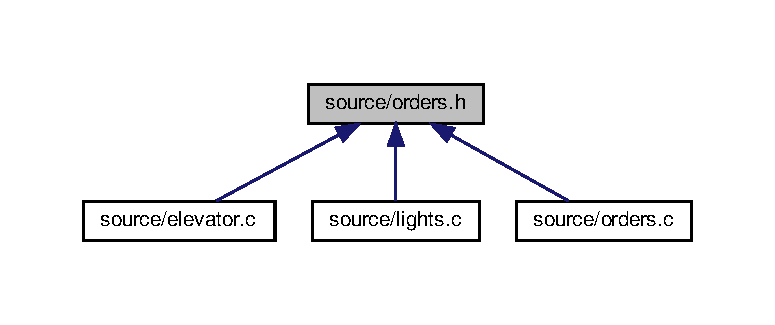
\includegraphics[width=350pt]{orders_8h__dep__incl}
\end{center}
\end{figure}
\subsection*{Functions}
\begin{DoxyCompactItemize}
\item 
int \hyperlink{orders_8h_ac426009b9dd5bd9bc76949a454a320a6}{get\+\_\+current\+\_\+direction} ()
\begin{DoxyCompactList}\small\item\em Gets the current direction. \end{DoxyCompactList}\item 
void \hyperlink{orders_8h_acf6f3f01ccc5d2cc5678499e4a992400}{set\+\_\+current\+\_\+direction} (int direction)
\begin{DoxyCompactList}\small\item\em Sets current\+\_\+direction to {\ttfamily direction} . \end{DoxyCompactList}\item 
int \hyperlink{orders_8h_acf20a30f171233e040ea4b4b2e5f4a46}{get\+\_\+order\+\_\+at\+\_\+floor} (int floor)
\begin{DoxyCompactList}\small\item\em Gets the value of elevator\+\_\+order\+\_\+array with index {\ttfamily floor} . \end{DoxyCompactList}\item 
void \hyperlink{orders_8h_ac6cd7c279c95b7a210719dffada982d8}{set\+\_\+order\+\_\+at\+\_\+floor} (int floor, int order)
\begin{DoxyCompactList}\small\item\em Sets the value of elevator\+\_\+order\+\_\+array with index {\ttfamily floor} to {\ttfamily order} . \end{DoxyCompactList}\item 
void \hyperlink{orders_8h_ae53d74727711dab412fb4c01aaa029da}{set\+\_\+order\+\_\+up} ()
\begin{DoxyCompactList}\small\item\em Updates elevator\+\_\+order\+\_\+array if any of the order up buttons are pressed. \end{DoxyCompactList}\item 
void \hyperlink{orders_8h_a4cf3627d1c6a40e9af29458da858558b}{set\+\_\+order\+\_\+down} ()
\begin{DoxyCompactList}\small\item\em Updates elevator\+\_\+order\+\_\+array if any of the order down buttons are pressed. \end{DoxyCompactList}\item 
void \hyperlink{orders_8h_ad81206d15e03830095bf5012a7ec48e0}{set\+\_\+order\+\_\+inside} ()
\begin{DoxyCompactList}\small\item\em Updates elevator\+\_\+order\+\_\+array if any of the order inside buttons are pressed. \end{DoxyCompactList}\item 
void \hyperlink{orders_8h_a60ab7f01650e26035d6ed4c623d3659d}{handle\+\_\+orders} ()
\begin{DoxyCompactList}\small\item\em Updates elevator\+\_\+order\+\_\+array if any order buttons are pressed. \end{DoxyCompactList}\item 
int \hyperlink{orders_8h_ae1f8082a7b2f16cecfd3ace6d8c6d73f}{check\+\_\+orders\+\_\+above} (int starting\+\_\+point)
\begin{DoxyCompactList}\small\item\em Checks if there are any order above {\ttfamily starting\+\_\+point} . \end{DoxyCompactList}\item 
int \hyperlink{orders_8h_a46e249c28b02726e1867ae718644a33f}{check\+\_\+orders\+\_\+below} (int starting\+\_\+point)
\begin{DoxyCompactList}\small\item\em Checks if there are any order below {\ttfamily starting\+\_\+point} . \end{DoxyCompactList}\item 
int \hyperlink{orders_8h_a5a309ac4f781a8b05b200d09a16987dc}{get\+\_\+order\+\_\+count} ()
\begin{DoxyCompactList}\small\item\em Gets the total amount of unattended orders. \end{DoxyCompactList}\item 
void \hyperlink{orders_8h_a1ae3ab02b290c9ba95abb9a3fc5bdbd1}{update\+\_\+current\+\_\+direction} ()
\begin{DoxyCompactList}\small\item\em Updates current\+\_\+direction based on existing orders, current\+\_\+direction and last\+\_\+direction. \end{DoxyCompactList}\item 
int \hyperlink{orders_8h_a263178a16b07955e026ff65f9f246d60}{check\+\_\+up\+\_\+at\+\_\+floor} ()
\begin{DoxyCompactList}\small\item\em Checks if there are any up orders at the current floor. \end{DoxyCompactList}\item 
int \hyperlink{orders_8h_a6a754d33f3fb49024aea10f590f25dea}{check\+\_\+down\+\_\+at\+\_\+floor} ()
\begin{DoxyCompactList}\small\item\em Checks if there are any down orders at the current floor. \end{DoxyCompactList}\item 
int \hyperlink{orders_8h_aa2814fca8943e13c07a75aca10cc4517}{check\+\_\+both\+\_\+or\+\_\+cab\+\_\+at\+\_\+floor} ()
\begin{DoxyCompactList}\small\item\em Checks if there are any cab orders or up and down orders simultaneously at the current floor. \end{DoxyCompactList}\item 
int \hyperlink{orders_8h_a0be2dc6cef3d1e0ebcc153b9b0f78d93}{check\+\_\+arrival} ()
\begin{DoxyCompactList}\small\item\em Checks if the elevator has arrived at a floor with an order that needs to be attended. \end{DoxyCompactList}\item 
void \hyperlink{orders_8h_a6206e5203639ca23d84820e2ffb108a3}{clear\+\_\+all\+\_\+orders} ()
\begin{DoxyCompactList}\small\item\em Clears all existing orders in elevator\+\_\+order\+\_\+array. \end{DoxyCompactList}\item 
void \hyperlink{orders_8h_a246f5cd101e20bda3d5f2607f8e56f0c}{print\+\_\+all\+\_\+orders} ()
\begin{DoxyCompactList}\small\item\em Prints all existing orders in elevator\+\_\+order\+\_\+array. \end{DoxyCompactList}\item 
int \hyperlink{orders_8h_a47efe536e1dd0d64e2f4edf1af2345b4}{bool\+\_\+order\+\_\+at\+\_\+floor} (int floor)
\begin{DoxyCompactList}\small\item\em Checks if there are any orders at at {\ttfamily floor} . \end{DoxyCompactList}\end{DoxyCompactItemize}


\subsection{Detailed Description}
Order handling, including the queue system. 



\subsection{Function Documentation}
\mbox{\Hypertarget{orders_8h_a47efe536e1dd0d64e2f4edf1af2345b4}\label{orders_8h_a47efe536e1dd0d64e2f4edf1af2345b4}} 
\index{orders.\+h@{orders.\+h}!bool\+\_\+order\+\_\+at\+\_\+floor@{bool\+\_\+order\+\_\+at\+\_\+floor}}
\index{bool\+\_\+order\+\_\+at\+\_\+floor@{bool\+\_\+order\+\_\+at\+\_\+floor}!orders.\+h@{orders.\+h}}
\subsubsection{\texorpdfstring{bool\+\_\+order\+\_\+at\+\_\+floor()}{bool\_order\_at\_floor()}}
{\footnotesize\ttfamily int bool\+\_\+order\+\_\+at\+\_\+floor (\begin{DoxyParamCaption}\item[{int}]{floor }\end{DoxyParamCaption})}



Checks if there are any orders at at {\ttfamily floor} . 


\begin{DoxyParams}{Parameters}
{\em floor} & \\
\hline
\end{DoxyParams}
\begin{DoxyReturn}{Returns}
Return 1 if order at requested floor. Return 0 otherwise. 
\end{DoxyReturn}


Definition at line 185 of file orders.\+c.

\mbox{\Hypertarget{orders_8h_a0be2dc6cef3d1e0ebcc153b9b0f78d93}\label{orders_8h_a0be2dc6cef3d1e0ebcc153b9b0f78d93}} 
\index{orders.\+h@{orders.\+h}!check\+\_\+arrival@{check\+\_\+arrival}}
\index{check\+\_\+arrival@{check\+\_\+arrival}!orders.\+h@{orders.\+h}}
\subsubsection{\texorpdfstring{check\+\_\+arrival()}{check\_arrival()}}
{\footnotesize\ttfamily int check\+\_\+arrival (\begin{DoxyParamCaption}{ }\end{DoxyParamCaption})}



Checks if the elevator has arrived at a floor with an order that needs to be attended. 

\begin{DoxyReturn}{Returns}
Return 1 if arrived at floor with order. Return 0 otherwise. 
\end{DoxyReturn}


Definition at line 154 of file orders.\+c.

\mbox{\Hypertarget{orders_8h_aa2814fca8943e13c07a75aca10cc4517}\label{orders_8h_aa2814fca8943e13c07a75aca10cc4517}} 
\index{orders.\+h@{orders.\+h}!check\+\_\+both\+\_\+or\+\_\+cab\+\_\+at\+\_\+floor@{check\+\_\+both\+\_\+or\+\_\+cab\+\_\+at\+\_\+floor}}
\index{check\+\_\+both\+\_\+or\+\_\+cab\+\_\+at\+\_\+floor@{check\+\_\+both\+\_\+or\+\_\+cab\+\_\+at\+\_\+floor}!orders.\+h@{orders.\+h}}
\subsubsection{\texorpdfstring{check\+\_\+both\+\_\+or\+\_\+cab\+\_\+at\+\_\+floor()}{check\_both\_or\_cab\_at\_floor()}}
{\footnotesize\ttfamily int check\+\_\+both\+\_\+or\+\_\+cab\+\_\+at\+\_\+floor (\begin{DoxyParamCaption}{ }\end{DoxyParamCaption})}



Checks if there are any cab orders or up and down orders simultaneously at the current floor. 

\begin{DoxyReturn}{Returns}
Return 1 if cab order or up and down order at floor. Return 0 otherwise. 
\end{DoxyReturn}


Definition at line 145 of file orders.\+c.

\mbox{\Hypertarget{orders_8h_a6a754d33f3fb49024aea10f590f25dea}\label{orders_8h_a6a754d33f3fb49024aea10f590f25dea}} 
\index{orders.\+h@{orders.\+h}!check\+\_\+down\+\_\+at\+\_\+floor@{check\+\_\+down\+\_\+at\+\_\+floor}}
\index{check\+\_\+down\+\_\+at\+\_\+floor@{check\+\_\+down\+\_\+at\+\_\+floor}!orders.\+h@{orders.\+h}}
\subsubsection{\texorpdfstring{check\+\_\+down\+\_\+at\+\_\+floor()}{check\_down\_at\_floor()}}
{\footnotesize\ttfamily int check\+\_\+down\+\_\+at\+\_\+floor (\begin{DoxyParamCaption}{ }\end{DoxyParamCaption})}



Checks if there are any down orders at the current floor. 

\begin{DoxyReturn}{Returns}
Return 1 if down order at floor. Return 0 otherwise. 
\end{DoxyReturn}


Definition at line 136 of file orders.\+c.

\mbox{\Hypertarget{orders_8h_ae1f8082a7b2f16cecfd3ace6d8c6d73f}\label{orders_8h_ae1f8082a7b2f16cecfd3ace6d8c6d73f}} 
\index{orders.\+h@{orders.\+h}!check\+\_\+orders\+\_\+above@{check\+\_\+orders\+\_\+above}}
\index{check\+\_\+orders\+\_\+above@{check\+\_\+orders\+\_\+above}!orders.\+h@{orders.\+h}}
\subsubsection{\texorpdfstring{check\+\_\+orders\+\_\+above()}{check\_orders\_above()}}
{\footnotesize\ttfamily int check\+\_\+orders\+\_\+above (\begin{DoxyParamCaption}\item[{int}]{starting\+\_\+point }\end{DoxyParamCaption})}



Checks if there are any order above {\ttfamily starting\+\_\+point} . 


\begin{DoxyParams}{Parameters}
{\em starting\+\_\+point} & \\
\hline
\end{DoxyParams}
\begin{DoxyReturn}{Returns}
Return 1 if there are orders above. Return 0 otherwise. 
\end{DoxyReturn}


Definition at line 70 of file orders.\+c.

\mbox{\Hypertarget{orders_8h_a46e249c28b02726e1867ae718644a33f}\label{orders_8h_a46e249c28b02726e1867ae718644a33f}} 
\index{orders.\+h@{orders.\+h}!check\+\_\+orders\+\_\+below@{check\+\_\+orders\+\_\+below}}
\index{check\+\_\+orders\+\_\+below@{check\+\_\+orders\+\_\+below}!orders.\+h@{orders.\+h}}
\subsubsection{\texorpdfstring{check\+\_\+orders\+\_\+below()}{check\_orders\_below()}}
{\footnotesize\ttfamily int check\+\_\+orders\+\_\+below (\begin{DoxyParamCaption}\item[{int}]{starting\+\_\+point }\end{DoxyParamCaption})}



Checks if there are any order below {\ttfamily starting\+\_\+point} . 


\begin{DoxyParams}{Parameters}
{\em starting\+\_\+point} & \\
\hline
\end{DoxyParams}
\begin{DoxyReturn}{Returns}
Return 1 if there are orders below. Return 0 otherwise. 
\end{DoxyReturn}


Definition at line 81 of file orders.\+c.

\mbox{\Hypertarget{orders_8h_a263178a16b07955e026ff65f9f246d60}\label{orders_8h_a263178a16b07955e026ff65f9f246d60}} 
\index{orders.\+h@{orders.\+h}!check\+\_\+up\+\_\+at\+\_\+floor@{check\+\_\+up\+\_\+at\+\_\+floor}}
\index{check\+\_\+up\+\_\+at\+\_\+floor@{check\+\_\+up\+\_\+at\+\_\+floor}!orders.\+h@{orders.\+h}}
\subsubsection{\texorpdfstring{check\+\_\+up\+\_\+at\+\_\+floor()}{check\_up\_at\_floor()}}
{\footnotesize\ttfamily int check\+\_\+up\+\_\+at\+\_\+floor (\begin{DoxyParamCaption}{ }\end{DoxyParamCaption})}



Checks if there are any up orders at the current floor. 

\begin{DoxyReturn}{Returns}
Return 1 if up order at floor. Return 0 otherwise. 
\end{DoxyReturn}


Definition at line 127 of file orders.\+c.

\mbox{\Hypertarget{orders_8h_a6206e5203639ca23d84820e2ffb108a3}\label{orders_8h_a6206e5203639ca23d84820e2ffb108a3}} 
\index{orders.\+h@{orders.\+h}!clear\+\_\+all\+\_\+orders@{clear\+\_\+all\+\_\+orders}}
\index{clear\+\_\+all\+\_\+orders@{clear\+\_\+all\+\_\+orders}!orders.\+h@{orders.\+h}}
\subsubsection{\texorpdfstring{clear\+\_\+all\+\_\+orders()}{clear\_all\_orders()}}
{\footnotesize\ttfamily void clear\+\_\+all\+\_\+orders (\begin{DoxyParamCaption}{ }\end{DoxyParamCaption})}



Clears all existing orders in elevator\+\_\+order\+\_\+array. 



Definition at line 173 of file orders.\+c.

\mbox{\Hypertarget{orders_8h_ac426009b9dd5bd9bc76949a454a320a6}\label{orders_8h_ac426009b9dd5bd9bc76949a454a320a6}} 
\index{orders.\+h@{orders.\+h}!get\+\_\+current\+\_\+direction@{get\+\_\+current\+\_\+direction}}
\index{get\+\_\+current\+\_\+direction@{get\+\_\+current\+\_\+direction}!orders.\+h@{orders.\+h}}
\subsubsection{\texorpdfstring{get\+\_\+current\+\_\+direction()}{get\_current\_direction()}}
{\footnotesize\ttfamily int get\+\_\+current\+\_\+direction (\begin{DoxyParamCaption}{ }\end{DoxyParamCaption})}



Gets the current direction. 

\begin{DoxyReturn}{Returns}
Return current\+\_\+direction. 
\end{DoxyReturn}


Definition at line 13 of file orders.\+c.

\mbox{\Hypertarget{orders_8h_acf20a30f171233e040ea4b4b2e5f4a46}\label{orders_8h_acf20a30f171233e040ea4b4b2e5f4a46}} 
\index{orders.\+h@{orders.\+h}!get\+\_\+order\+\_\+at\+\_\+floor@{get\+\_\+order\+\_\+at\+\_\+floor}}
\index{get\+\_\+order\+\_\+at\+\_\+floor@{get\+\_\+order\+\_\+at\+\_\+floor}!orders.\+h@{orders.\+h}}
\subsubsection{\texorpdfstring{get\+\_\+order\+\_\+at\+\_\+floor()}{get\_order\_at\_floor()}}
{\footnotesize\ttfamily int get\+\_\+order\+\_\+at\+\_\+floor (\begin{DoxyParamCaption}\item[{int}]{floor }\end{DoxyParamCaption})}



Gets the value of elevator\+\_\+order\+\_\+array with index {\ttfamily floor} . 


\begin{DoxyParams}{Parameters}
{\em floor} & \\
\hline
\end{DoxyParams}
\begin{DoxyReturn}{Returns}
Return the value of elevator\+\_\+order\+\_\+array with selected index. 
\end{DoxyReturn}


Definition at line 21 of file orders.\+c.

\mbox{\Hypertarget{orders_8h_a5a309ac4f781a8b05b200d09a16987dc}\label{orders_8h_a5a309ac4f781a8b05b200d09a16987dc}} 
\index{orders.\+h@{orders.\+h}!get\+\_\+order\+\_\+count@{get\+\_\+order\+\_\+count}}
\index{get\+\_\+order\+\_\+count@{get\+\_\+order\+\_\+count}!orders.\+h@{orders.\+h}}
\subsubsection{\texorpdfstring{get\+\_\+order\+\_\+count()}{get\_order\_count()}}
{\footnotesize\ttfamily int get\+\_\+order\+\_\+count (\begin{DoxyParamCaption}{ }\end{DoxyParamCaption})}



Gets the total amount of unattended orders. 

\begin{DoxyReturn}{Returns}
Return the total amount of unattended orders. 
\end{DoxyReturn}


Definition at line 92 of file orders.\+c.

\mbox{\Hypertarget{orders_8h_a60ab7f01650e26035d6ed4c623d3659d}\label{orders_8h_a60ab7f01650e26035d6ed4c623d3659d}} 
\index{orders.\+h@{orders.\+h}!handle\+\_\+orders@{handle\+\_\+orders}}
\index{handle\+\_\+orders@{handle\+\_\+orders}!orders.\+h@{orders.\+h}}
\subsubsection{\texorpdfstring{handle\+\_\+orders()}{handle\_orders()}}
{\footnotesize\ttfamily void handle\+\_\+orders (\begin{DoxyParamCaption}{ }\end{DoxyParamCaption})}



Updates elevator\+\_\+order\+\_\+array if any order buttons are pressed. 



Definition at line 64 of file orders.\+c.

\mbox{\Hypertarget{orders_8h_a246f5cd101e20bda3d5f2607f8e56f0c}\label{orders_8h_a246f5cd101e20bda3d5f2607f8e56f0c}} 
\index{orders.\+h@{orders.\+h}!print\+\_\+all\+\_\+orders@{print\+\_\+all\+\_\+orders}}
\index{print\+\_\+all\+\_\+orders@{print\+\_\+all\+\_\+orders}!orders.\+h@{orders.\+h}}
\subsubsection{\texorpdfstring{print\+\_\+all\+\_\+orders()}{print\_all\_orders()}}
{\footnotesize\ttfamily void print\+\_\+all\+\_\+orders (\begin{DoxyParamCaption}{ }\end{DoxyParamCaption})}



Prints all existing orders in elevator\+\_\+order\+\_\+array. 



Definition at line 179 of file orders.\+c.

\mbox{\Hypertarget{orders_8h_acf6f3f01ccc5d2cc5678499e4a992400}\label{orders_8h_acf6f3f01ccc5d2cc5678499e4a992400}} 
\index{orders.\+h@{orders.\+h}!set\+\_\+current\+\_\+direction@{set\+\_\+current\+\_\+direction}}
\index{set\+\_\+current\+\_\+direction@{set\+\_\+current\+\_\+direction}!orders.\+h@{orders.\+h}}
\subsubsection{\texorpdfstring{set\+\_\+current\+\_\+direction()}{set\_current\_direction()}}
{\footnotesize\ttfamily void set\+\_\+current\+\_\+direction (\begin{DoxyParamCaption}\item[{int}]{direction }\end{DoxyParamCaption})}



Sets current\+\_\+direction to {\ttfamily direction} . 


\begin{DoxyParams}{Parameters}
{\em direction} & \\
\hline
\end{DoxyParams}


Definition at line 17 of file orders.\+c.

\mbox{\Hypertarget{orders_8h_ac6cd7c279c95b7a210719dffada982d8}\label{orders_8h_ac6cd7c279c95b7a210719dffada982d8}} 
\index{orders.\+h@{orders.\+h}!set\+\_\+order\+\_\+at\+\_\+floor@{set\+\_\+order\+\_\+at\+\_\+floor}}
\index{set\+\_\+order\+\_\+at\+\_\+floor@{set\+\_\+order\+\_\+at\+\_\+floor}!orders.\+h@{orders.\+h}}
\subsubsection{\texorpdfstring{set\+\_\+order\+\_\+at\+\_\+floor()}{set\_order\_at\_floor()}}
{\footnotesize\ttfamily void set\+\_\+order\+\_\+at\+\_\+floor (\begin{DoxyParamCaption}\item[{int}]{floor,  }\item[{int}]{order }\end{DoxyParamCaption})}



Sets the value of elevator\+\_\+order\+\_\+array with index {\ttfamily floor} to {\ttfamily order} . 


\begin{DoxyParams}{Parameters}
{\em floor} & \\
\hline
{\em order} & \\
\hline
\end{DoxyParams}


Definition at line 25 of file orders.\+c.

\mbox{\Hypertarget{orders_8h_a4cf3627d1c6a40e9af29458da858558b}\label{orders_8h_a4cf3627d1c6a40e9af29458da858558b}} 
\index{orders.\+h@{orders.\+h}!set\+\_\+order\+\_\+down@{set\+\_\+order\+\_\+down}}
\index{set\+\_\+order\+\_\+down@{set\+\_\+order\+\_\+down}!orders.\+h@{orders.\+h}}
\subsubsection{\texorpdfstring{set\+\_\+order\+\_\+down()}{set\_order\_down()}}
{\footnotesize\ttfamily void set\+\_\+order\+\_\+down (\begin{DoxyParamCaption}{ }\end{DoxyParamCaption})}



Updates elevator\+\_\+order\+\_\+array if any of the order down buttons are pressed. 



Definition at line 43 of file orders.\+c.

\mbox{\Hypertarget{orders_8h_ad81206d15e03830095bf5012a7ec48e0}\label{orders_8h_ad81206d15e03830095bf5012a7ec48e0}} 
\index{orders.\+h@{orders.\+h}!set\+\_\+order\+\_\+inside@{set\+\_\+order\+\_\+inside}}
\index{set\+\_\+order\+\_\+inside@{set\+\_\+order\+\_\+inside}!orders.\+h@{orders.\+h}}
\subsubsection{\texorpdfstring{set\+\_\+order\+\_\+inside()}{set\_order\_inside()}}
{\footnotesize\ttfamily void set\+\_\+order\+\_\+inside (\begin{DoxyParamCaption}{ }\end{DoxyParamCaption})}



Updates elevator\+\_\+order\+\_\+array if any of the order inside buttons are pressed. 



Definition at line 56 of file orders.\+c.

\mbox{\Hypertarget{orders_8h_ae53d74727711dab412fb4c01aaa029da}\label{orders_8h_ae53d74727711dab412fb4c01aaa029da}} 
\index{orders.\+h@{orders.\+h}!set\+\_\+order\+\_\+up@{set\+\_\+order\+\_\+up}}
\index{set\+\_\+order\+\_\+up@{set\+\_\+order\+\_\+up}!orders.\+h@{orders.\+h}}
\subsubsection{\texorpdfstring{set\+\_\+order\+\_\+up()}{set\_order\_up()}}
{\footnotesize\ttfamily void set\+\_\+order\+\_\+up (\begin{DoxyParamCaption}{ }\end{DoxyParamCaption})}



Updates elevator\+\_\+order\+\_\+array if any of the order up buttons are pressed. 



Definition at line 30 of file orders.\+c.

\mbox{\Hypertarget{orders_8h_a1ae3ab02b290c9ba95abb9a3fc5bdbd1}\label{orders_8h_a1ae3ab02b290c9ba95abb9a3fc5bdbd1}} 
\index{orders.\+h@{orders.\+h}!update\+\_\+current\+\_\+direction@{update\+\_\+current\+\_\+direction}}
\index{update\+\_\+current\+\_\+direction@{update\+\_\+current\+\_\+direction}!orders.\+h@{orders.\+h}}
\subsubsection{\texorpdfstring{update\+\_\+current\+\_\+direction()}{update\_current\_direction()}}
{\footnotesize\ttfamily void update\+\_\+current\+\_\+direction (\begin{DoxyParamCaption}{ }\end{DoxyParamCaption})}



Updates current\+\_\+direction based on existing orders, current\+\_\+direction and last\+\_\+direction. 



Definition at line 102 of file orders.\+c.


\hypertarget{timer_8c}{}\section{source/timer.c File Reference}
\label{timer_8c}\index{source/timer.\+c@{source/timer.\+c}}
{\ttfamily \#include \char`\"{}timer.\+h\char`\"{}}\newline
{\ttfamily \#include $<$stdio.\+h$>$}\newline
{\ttfamily \#include $<$stdlib.\+h$>$}\newline
{\ttfamily \#include $<$time.\+h$>$}\newline
Include dependency graph for timer.\+c\+:
\nopagebreak
\begin{figure}[H]
\begin{center}
\leavevmode
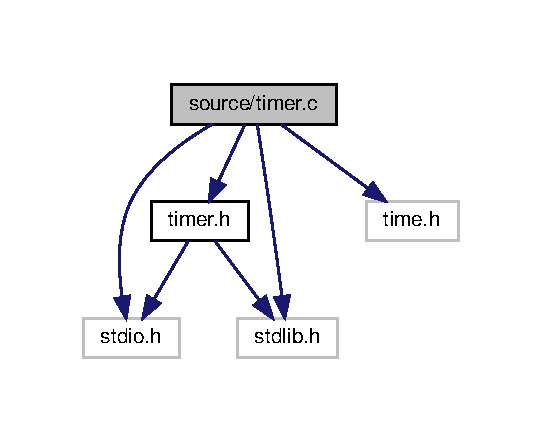
\includegraphics[width=260pt]{timer_8c__incl}
\end{center}
\end{figure}
\subsection*{Functions}
\begin{DoxyCompactItemize}
\item 
void \hyperlink{timer_8c_a22921481d2faa838e662c9f46ded0402}{timer\+\_\+start\+\_\+timer} (int msec)
\begin{DoxyCompactList}\small\item\em Starts a timer that expires after {\ttfamily msec} seconds. \end{DoxyCompactList}\item 
int \hyperlink{timer_8c_abecf7c61d9bc3306e5d1238dea0daad7}{timer\+\_\+check\+\_\+expired} ()
\begin{DoxyCompactList}\small\item\em Checks if the timer has expired. \end{DoxyCompactList}\item 
void \hyperlink{timer_8c_a4d54d420a1c989573e113106557d7489}{timer\+\_\+print\+\_\+current\+\_\+time} ()
\begin{DoxyCompactList}\small\item\em Prints the elapsed time since the timer was started. \end{DoxyCompactList}\item 
void \hyperlink{timer_8c_a94f034f9dcd8673bc63442cbda10b0f8}{timer\+\_\+test\+\_\+timer} ()
\begin{DoxyCompactList}\small\item\em Starts a 5 second timer and prints the elapsed time. \end{DoxyCompactList}\end{DoxyCompactItemize}


\subsection{Function Documentation}
\mbox{\Hypertarget{timer_8c_abecf7c61d9bc3306e5d1238dea0daad7}\label{timer_8c_abecf7c61d9bc3306e5d1238dea0daad7}} 
\index{timer.\+c@{timer.\+c}!timer\+\_\+check\+\_\+expired@{timer\+\_\+check\+\_\+expired}}
\index{timer\+\_\+check\+\_\+expired@{timer\+\_\+check\+\_\+expired}!timer.\+c@{timer.\+c}}
\subsubsection{\texorpdfstring{timer\+\_\+check\+\_\+expired()}{timer\_check\_expired()}}
{\footnotesize\ttfamily int timer\+\_\+check\+\_\+expired (\begin{DoxyParamCaption}{ }\end{DoxyParamCaption})}



Checks if the timer has expired. 

\begin{DoxyReturn}{Returns}
Return 1 if the timer has expired. Return 0 otherwise. 
\end{DoxyReturn}


Definition at line 15 of file timer.\+c.

\mbox{\Hypertarget{timer_8c_a4d54d420a1c989573e113106557d7489}\label{timer_8c_a4d54d420a1c989573e113106557d7489}} 
\index{timer.\+c@{timer.\+c}!timer\+\_\+print\+\_\+current\+\_\+time@{timer\+\_\+print\+\_\+current\+\_\+time}}
\index{timer\+\_\+print\+\_\+current\+\_\+time@{timer\+\_\+print\+\_\+current\+\_\+time}!timer.\+c@{timer.\+c}}
\subsubsection{\texorpdfstring{timer\+\_\+print\+\_\+current\+\_\+time()}{timer\_print\_current\_time()}}
{\footnotesize\ttfamily void timer\+\_\+print\+\_\+current\+\_\+time (\begin{DoxyParamCaption}{ }\end{DoxyParamCaption})}



Prints the elapsed time since the timer was started. 



Definition at line 26 of file timer.\+c.

\mbox{\Hypertarget{timer_8c_a22921481d2faa838e662c9f46ded0402}\label{timer_8c_a22921481d2faa838e662c9f46ded0402}} 
\index{timer.\+c@{timer.\+c}!timer\+\_\+start\+\_\+timer@{timer\+\_\+start\+\_\+timer}}
\index{timer\+\_\+start\+\_\+timer@{timer\+\_\+start\+\_\+timer}!timer.\+c@{timer.\+c}}
\subsubsection{\texorpdfstring{timer\+\_\+start\+\_\+timer()}{timer\_start\_timer()}}
{\footnotesize\ttfamily void timer\+\_\+start\+\_\+timer (\begin{DoxyParamCaption}\item[{int}]{msec }\end{DoxyParamCaption})}



Starts a timer that expires after {\ttfamily msec} seconds. 


\begin{DoxyParams}{Parameters}
{\em msec} & \\
\hline
\end{DoxyParams}


Definition at line 10 of file timer.\+c.

\mbox{\Hypertarget{timer_8c_a94f034f9dcd8673bc63442cbda10b0f8}\label{timer_8c_a94f034f9dcd8673bc63442cbda10b0f8}} 
\index{timer.\+c@{timer.\+c}!timer\+\_\+test\+\_\+timer@{timer\+\_\+test\+\_\+timer}}
\index{timer\+\_\+test\+\_\+timer@{timer\+\_\+test\+\_\+timer}!timer.\+c@{timer.\+c}}
\subsubsection{\texorpdfstring{timer\+\_\+test\+\_\+timer()}{timer\_test\_timer()}}
{\footnotesize\ttfamily void timer\+\_\+test\+\_\+timer (\begin{DoxyParamCaption}{ }\end{DoxyParamCaption})}



Starts a 5 second timer and prints the elapsed time. 



Definition at line 31 of file timer.\+c.


\hypertarget{timer_8h}{}\section{source/timer.h File Reference}
\label{timer_8h}\index{source/timer.\+h@{source/timer.\+h}}


Time functions.  


{\ttfamily \#include $<$stdio.\+h$>$}\newline
{\ttfamily \#include $<$stdlib.\+h$>$}\newline
Include dependency graph for timer.\+h\+:\nopagebreak
\begin{figure}[H]
\begin{center}
\leavevmode
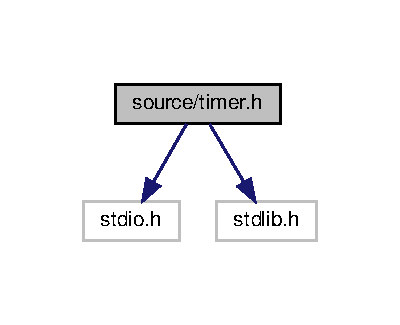
\includegraphics[width=192pt]{timer_8h__incl}
\end{center}
\end{figure}
This graph shows which files directly or indirectly include this file\+:\nopagebreak
\begin{figure}[H]
\begin{center}
\leavevmode
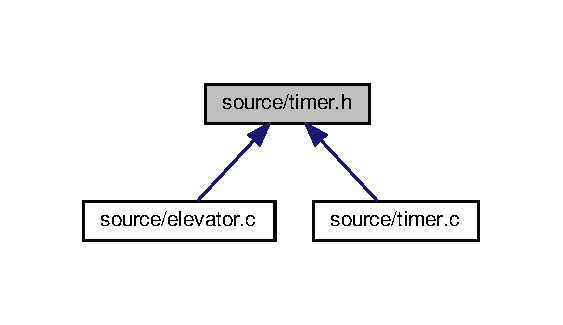
\includegraphics[width=270pt]{timer_8h__dep__incl}
\end{center}
\end{figure}
\subsection*{Functions}
\begin{DoxyCompactItemize}
\item 
void \hyperlink{timer_8h_a22921481d2faa838e662c9f46ded0402}{timer\+\_\+start\+\_\+timer} (int msec)
\begin{DoxyCompactList}\small\item\em Starts a timer that expires after {\ttfamily msec} seconds. \end{DoxyCompactList}\item 
int \hyperlink{timer_8h_abecf7c61d9bc3306e5d1238dea0daad7}{timer\+\_\+check\+\_\+expired} ()
\begin{DoxyCompactList}\small\item\em Checks if the timer has expired. \end{DoxyCompactList}\item 
void \hyperlink{timer_8h_a4d54d420a1c989573e113106557d7489}{timer\+\_\+print\+\_\+current\+\_\+time} ()
\begin{DoxyCompactList}\small\item\em Prints the elapsed time since the timer was started. \end{DoxyCompactList}\item 
void \hyperlink{timer_8h_a94f034f9dcd8673bc63442cbda10b0f8}{timer\+\_\+test\+\_\+timer} ()
\begin{DoxyCompactList}\small\item\em Starts a 5 second timer and prints the elapsed time. \end{DoxyCompactList}\end{DoxyCompactItemize}


\subsection{Detailed Description}
Time functions. 

Functions used to keep doors open for 3 seconds etc. 

\subsection{Function Documentation}
\mbox{\Hypertarget{timer_8h_abecf7c61d9bc3306e5d1238dea0daad7}\label{timer_8h_abecf7c61d9bc3306e5d1238dea0daad7}} 
\index{timer.\+h@{timer.\+h}!timer\+\_\+check\+\_\+expired@{timer\+\_\+check\+\_\+expired}}
\index{timer\+\_\+check\+\_\+expired@{timer\+\_\+check\+\_\+expired}!timer.\+h@{timer.\+h}}
\subsubsection{\texorpdfstring{timer\+\_\+check\+\_\+expired()}{timer\_check\_expired()}}
{\footnotesize\ttfamily int timer\+\_\+check\+\_\+expired (\begin{DoxyParamCaption}{ }\end{DoxyParamCaption})}



Checks if the timer has expired. 

\begin{DoxyReturn}{Returns}
Return 1 if the timer has expired. Return 0 otherwise. 
\end{DoxyReturn}


Definition at line 15 of file timer.\+c.

\mbox{\Hypertarget{timer_8h_a4d54d420a1c989573e113106557d7489}\label{timer_8h_a4d54d420a1c989573e113106557d7489}} 
\index{timer.\+h@{timer.\+h}!timer\+\_\+print\+\_\+current\+\_\+time@{timer\+\_\+print\+\_\+current\+\_\+time}}
\index{timer\+\_\+print\+\_\+current\+\_\+time@{timer\+\_\+print\+\_\+current\+\_\+time}!timer.\+h@{timer.\+h}}
\subsubsection{\texorpdfstring{timer\+\_\+print\+\_\+current\+\_\+time()}{timer\_print\_current\_time()}}
{\footnotesize\ttfamily void timer\+\_\+print\+\_\+current\+\_\+time (\begin{DoxyParamCaption}{ }\end{DoxyParamCaption})}



Prints the elapsed time since the timer was started. 



Definition at line 26 of file timer.\+c.

\mbox{\Hypertarget{timer_8h_a22921481d2faa838e662c9f46ded0402}\label{timer_8h_a22921481d2faa838e662c9f46ded0402}} 
\index{timer.\+h@{timer.\+h}!timer\+\_\+start\+\_\+timer@{timer\+\_\+start\+\_\+timer}}
\index{timer\+\_\+start\+\_\+timer@{timer\+\_\+start\+\_\+timer}!timer.\+h@{timer.\+h}}
\subsubsection{\texorpdfstring{timer\+\_\+start\+\_\+timer()}{timer\_start\_timer()}}
{\footnotesize\ttfamily void timer\+\_\+start\+\_\+timer (\begin{DoxyParamCaption}\item[{int}]{msec }\end{DoxyParamCaption})}



Starts a timer that expires after {\ttfamily msec} seconds. 


\begin{DoxyParams}{Parameters}
{\em msec} & \\
\hline
\end{DoxyParams}


Definition at line 10 of file timer.\+c.

\mbox{\Hypertarget{timer_8h_a94f034f9dcd8673bc63442cbda10b0f8}\label{timer_8h_a94f034f9dcd8673bc63442cbda10b0f8}} 
\index{timer.\+h@{timer.\+h}!timer\+\_\+test\+\_\+timer@{timer\+\_\+test\+\_\+timer}}
\index{timer\+\_\+test\+\_\+timer@{timer\+\_\+test\+\_\+timer}!timer.\+h@{timer.\+h}}
\subsubsection{\texorpdfstring{timer\+\_\+test\+\_\+timer()}{timer\_test\_timer()}}
{\footnotesize\ttfamily void timer\+\_\+test\+\_\+timer (\begin{DoxyParamCaption}{ }\end{DoxyParamCaption})}



Starts a 5 second timer and prints the elapsed time. 



Definition at line 31 of file timer.\+c.


%--- End generated contents ---

% Index
\backmatter
\newpage
\phantomsection
\clearemptydoublepage
\addcontentsline{toc}{chapter}{Index}
\printindex

\end{document}
